\documentclass[12pt]{article}

%% Math
\usepackage{amsmath}  % for math formulas
\usepackage{amssymb}  % for math symbols
\usepackage{bm}
\renewcommand{\vec}[1]{\bm{#1}} %% define vector notation

%% Tables
\usepackage{rotating} % enable sidewaystable
\usepackage{longtable} % used for long tables of data in appendix
\usepackage{booktabs}  % also for long tables of data in appendix
\usepackage{subfig}
%% Figures
\usepackage{graphicx}
%% all fig. legends on a separate page
%% http://tex.stackexchange.com/q/30477/1783
\usepackage{caption}
\usepackage{letltxmacro}% http://ctan.org/pkg/letltxmacro
\captionsetup{labelsep=none}
\DeclareCaptionTextFormat{none}{} \captionsetup{labelsep=none,textformat=none}

%% Text layout
\usepackage{setspace} 
\usepackage{geometry}
\geometry{verbose,a4paper,tmargin=2.4cm,bmargin=2.4cm,lmargin=2.4cm,rmargin=2.4cm}
\usepackage{lineno}
\linenumbers
\usepackage{Sweave}% use of Sweave with R code
\usepackage{natbib}
\bibliographystyle{ecology}


\date{} % Leave date blank
\begin{document}

\begin{flushleft}
\begin{spacing}{1.9}


{\Large Title: \textbf{Facilitating feedbacks between field measurements and ecosystem models}}

Running Title: \textbf{Feedbacks between measurements and models}

David~S. LeBauer$^{1,\ast}$
Dan Wang$^{1}$
Katherine~T. Richter$^{2}$
Carl~C. Davidson$^{2}$
Michael~C. Dietze$^{1,2}$
\\
\vspace{1em}
$^1$ Energy Biosciences Institute, $^2$ Department of Plant Biology, University of Illinois, Urbana, Illinois, USA
\\
\vspace{1em}
$^\ast$ Corresponding author \\ Telephone: (949) 433-7410 \\ Fax: (217) 244-3637 \\ E-mail: dlebauer@illinois.edu 

\newpage

\section*{Abstract} % 350 word limit
Ecological models help us understand how ecosystems function, predict responses to global change, and identify future research needs. 
However, widespread use of models is limited by the technical challenges of model-data synthesis and information management. 
 To address these challenges, we present a ecoinformatic workflow, the Predictive Ecosystem Analyzer (PEcAn), that facilitates model analysis. 
 Herein we describe the PEcAn modules that synthesize plant trait data to estimate model parameters, propagate parameter uncertainties through to model output, and evaluate the contribution of each parameter to model uncertainty. 
 We illustrate a comprehensive approach to the estimation of parameter values, starting with a statement of prior knowledge that is refined by species level data using Bayesian meta-analysis; this is the first use of a rigorous meta-analysis to inform the parameters of a mechanistic ecosystem model. 
 Parameter uncertainty is propagated using ensemble methods to estimate model uncertainty. 
Variance decomposition allows us to quantify the contribution of each parameter to model uncertainty; this information can be used to prioritize subsequent data collection.
 By streamlining the use of models and focusing efforts to identify and constrain the dominant sources of uncertainty in model output, the approach used by PEcAn can speed scientific progress.

 We demonstrate PEcAn's ability to incorporate data to reduce uncertainty in productivity of a perennial grass monoculture (\textit{Panicum virgatum} L.) modeled by the Ecosystem Demography model. 
 Prior estimates were specified for fifteen model parameters, and species-level data were available for seven of these. 
 Meta-analysis of species-level data substantially reduced the contribution of three parameters (specific leaf area [SLA], maximum carboxylation rate, and stomatal slope) to overall model uncertainty. 
 By contrast, root turnover rate, root respiration rate, and leaf width had little effect on model output, therefore trait data had little impact on model uncertainty. 
 For fine root allocation the decrease in parameter uncertainty was offset by an increase in model sensitivity.
 Remaining model uncertainty is driven by growth respiration, fine root allocation, leaf turnover rater, and SLA. 
By establishing robust channels of feedback between data collection and ecosystem modeling, PEcAn provides a framework for more efficient and integrative science.

\textbf{keywords:}  traits, ecoinformatics, ecophysiology, Ecosystem Demography, sensitivity analysis, variance decomposition, ecological forecast, Bayesian, meta-analysis, ecosystem model

\newpage

\section*{Introduction}
\label{sec:intro}

 In the face of unprecedented global change there is growing demand for predictions of ecosystem responses that provide actionable information for policy and management  \citep{clark2001efe}.
 Currently, the response of the terrestrial biosphere remains one of the largest sources of uncertainty in projections of climate change \citep{denman2007cbc}.
 This uncertainty comes from a combination of the uncertainties about our conceptual understanding of ecological systems, as captured by the structure and assumptions of the models used to make ecological forecasts, the uncertainties in the parameters of these models, and the uncertainties associated with the underlying data itself \citep{mcmahon2009pfu}.
 Reducing these uncertainties requires that we be able to synthesize existing information, efficiently identify the dominant sources of model uncertainty and target them with further field research.

 Despite the acknowledged importance of these activities, there is often a disconnect between model simulation and data collection.
 Both model-data synthesis and the investigation of uncertainty remain challenging, while the use of models to quantitatively inform data collection is extremely rare.
 Most modeling uses a single point estimate for each parameter, effectively treating each parameter value as completely certain.
 However, such point estimates do not account for the degree to which we understand a parameter based on observations.
 Furthermore, the rationale for a particular estimate is often unclear, as is the degree to which the estimate represents the process being observed or its representation in a model.
 In many cases, parameter values are chosen iteratively to ``tune'', or ``calibrate'' the model output to observations.
 A first step toward constraining model uncertainty is to account for uncertainty in model parameters instead of relying on point estimates.

 More rigorous approaches to estimating parameter values include model optimization and data assimilation \citep{medvigy2009mse,reichstein2003ims}, as well as Bayesian model-data fusion \citep{luo2011efd}.
 However, these approaches have generally started with uninformative or vague prior estimates of model parameters.
 These vague priors ignore available data that could directly inform parameter values; the most commonly used  vague prior distribution is a uniform.
 A uniform prior assigns equal probability to parameter values over its entire range, in many cases over many orders of magnitude.
 The use of such vague priors often exacerbates problems with equifinality \citep{richardson2005sme,williams2009ils,luo2009pic} which can produce unidentifiable parameters, as well as biologically unrealistic parameter sets that generate the right model output for the wrong reasons \citep{beven2001eda,beven2006met,williams2009ils}.
 % if there are strong parameter correlations, then providing constrains on a subset of parameters will reduce uncertainty about the other parameters, though we agree that this does not guarantee that the free parameters will converge on biologically realistic values.

 Another reason to use informed priors is to take advantage of one of the key strengths of the Bayesian paradigm: the ability to synthesize multiple sources of information in a rigorous and consistent framework.
 For example, plant traits related to leaf stoichiometry and photosynthetic capacity are often well constrained by previous research \citep{skillman2008qyv,reich2004gpp,wright2004wwl,wullschleger1993blc}, while other traits, such as root respiration rate, are more difficult to measure and data are sparse.
 Informed priors allow existing information to be formally integrated into model parameterization, even if there is no data for the particular species or plant functional type (PFT) being measured; the level of confidence in a parameter value is reflected in its variance.

 Models have rarely been used to quantify the value of data with respect to reducing uncertainty.
 Instead, data collection is often focused on answering specific questions in specific spatial, temporal, and taxonomic contexts.
 In these contexts, the value of a particular data set is based on the ability to answer a particular question.
 However, the same data set may have a very different value in the context of reducing model uncertainty.
 For example, a single data point used to inform a poorly understood but influential model parameter can reduce model uncertainty more than a large collection of data on a trait that is relatively well studied.
 In a modeling context, the value of an additional data point depends both on how much it constrains parameter uncertainty and the sensitivity of model output to the parameter. 
 Thus, the ability to comprehensively utilize available data in model parametrization can help to identify gaps in existing knowledge, improve the ability of models to account for current understanding, and inform data collection efforts by identifying the knowledge gaps most responsible for uncertainty.

 While the increasing sophistication of model-data fusion and uncertainty accounting is a critical step in the right direction, the complexity of such analyses can make models even less accessible.
 One of the reasons to make models more accessible, and to make them better at synthesizing existing data, is that they are fundamentally a formal, quantitative distillation of our current understanding of how a system works.
 As such, models can be used to identify gaps in our understanding and target further research.
 This feedback between models and data could be improved if models were routinely evaluated in a way that quantifies the value of data with respect to reducing uncertainty.
 We fundamentally believe that streamlining the informatics of modeling -- the need to track, process, and synthesize data and model output -- will make the development and application of ecological data and models more accessible, transparent, and relevant.

 In this paper we present the Predictive Ecosystem Analyzer (PEcAn) as a step toward meeting these objectives.
 PEcAn is a scientific workflow that manages the flows of data used and produced by ecological models, and that assists with model parametrization, error propagation, and error analysis.
 PEcAn accomplishes two goals: first, it synthesizes data and propagates uncertainty through an ecosystem model; second, it  places an information value on subsequent data collection that enables data collection that efficiently reduces uncertainty.
 In addition to quantifying the information content of any prediction or assessment, these techniques also help identify the gaps in our knowledge of ecological and biogeochemical processes \citep{saltelli2008gsa}.

 PEcAn addresses the challenge of synthesizing plant trait data from the literature in a way that accounts for the different scales and sources of uncertainty.
 Available data is synthesized using a Bayesian meta-analysis, and the meta-analysis posterior estimates of plant traits are used as parameters in an ecosystem model.

 A model ensemble is a set of model runs with parameter values drawn from the meta-analysis posteriors estimate of plant traits.
 Output from a model ensemble represents the posterior predictive distributions of ecosystem responses that account for trait parameter uncertainty (hereafter  ``model posterior'' refers to the ``model ensemble output'').
 Sensitivity analysis and variance decomposition help to determine which traits (model parameters) drive uncertainty in ecosystem response (model posterior) \citep{saltelli2008gsa,larocque2008uac}.
 These analyses help target parameters for further constraint with trait data, forming a critical feedback loop that drives further field research and provides an informative starting point for data assimilation.
 Here we illustrate an application of PEcAn to the assessment of aboveground yield in a perennial grass monoculture.

 In the sections below, we provide an overview of the components of PEcAn's integrated framework for data synthesis and ecological prediction. 
 We start with a description of the methods implemented in the workflow (Implementation).
 This includes descriptions of the database, Bayesian meta-analysis, ensemble analysis, sensitivity analysis, and variance decomposition.
 Finally we present an example of the application of the system (Application) to analyze the aboveground biomass of switchgrass (\emph{Panicum virgatum} L.), by the Ecosystem Demography model, version 2.1 (ED2) \citep{medvigy2009mse,moorcroft2001msv}.

\section*{Implementation}
\label{sec:implement}

\subsection*{PEcAn workflow}
  The Predictive Ecosystem Analyzer (PEcAn) manages the flow of information into and out of ecosystem models.%'p\overline{e}-,kan\\
 PEcAn is not a model itself, it is a scientific workflow consisting of discrete steps, or modules. 
 Individual modules are building blocks of the workflow, represented by the rectangles in Figure~\ref{fig:workflow}, while flows of information are represented by arrows. 
 This makes PEcAn an encapsulated, semi-automated system for model parametrization, error propagation, and analysis.
  
 A central objective of the PEcAn workflow is to make the entire modeling process transparent, reproducible, and adaptable to new questions  \citep[\textit{sensu} ][]{stodden2010rr,ellison2010rte}.
 To achieve this objective, PEcAn's adheres to ``best practice'' guidelines for ecological data management and provenance tracking \citep{jones2006nbi,michener2012ese}. 

 PEcAn uses a database to track data provenance and a settings file to control workflow analyses and model runs.
 The database records the site, date, management, species, and treatment information for each trait observation used in the meta-analysis.
 Settings related to the experimental design and computation are set and recorded in a separate file for each analysis.
   
 The PEcAn source code, as well as the inputs and output used in the analysis described below (see Application) are provided as an appendix.
 However, new users are encouraged to utilize the latest release available on the project web site (www.pecanproject.org).
 This site also provides a virtual machine and a web-interface that minimize the effort required to run PEcAn and begin using an ecosystem model.
 The PEcAn ``virtual machine'' provides all of the required software dependencies in a pre-configured desktop environment that can be run on any standard operating system using a freely available virtualization software such as VirtualBox (www.virtualbox.org/) or VmWare Player (www.vmware.com).
 The virtual machine minimizes the installation time and pre-requisite knowledge required to perform analyses, and can be used to support investigation, development, and education.
 The web interface is even easier to use, but does not provide access to all of PEcAn's functionality. 

 The PEcAn software is primarily written in R and developed in a Linux environment.
 It also relies on a MySQL database, bash, JAGS, and specialized R packages.
 PEcAn has a family of model-specific functions that manage the details of launching of model runs and reading model output.
 
 Although PEcAn does not depend on any specific model, it was developed to support ecosystem models that run in high-performance computing environments; for this reason, it is capable of running models locally, remotely, or through queuing systems regardless of whether PEcAn is compiled locally or run as a virtual machine.
 The PEcAn 1.1 release described herein runs with the Ecosystem Demography model, in addition, the current release also supports SIPNET \citep[][]{moore2008ets} and near term support for IBIS \citep{kucharik2000tpd}, DayCent \citep{parton1998dls}, and BioCro \citep{miguez2009smp} is under development.

\subsection*{Trait Database}
 
 Model parameters are associated with corresponding prior distributions, and in many cases, with species-level data.
 Both prior distributions and data are stored in a relational database (Appendix B).
 PEcAn directly accesses the database, which contains additional meta-data for each data set, including site descriptions, measurement conditions, experimental details, and citations.

\subsection*{Trait Priors}

 A fundamental component of the Bayesian approach to parameter estimation is the use of priors. 
 Priors formally incorporate knowledge of a parameter based on previous studies into a new analysis.
 In the current study, we leverage previously collected data from non-target species to place biologically informed constraint on the distribution of a plant trait parameter.
 When additional data for a specific species or plant functional type is available, priors are further constrained before being used as model parameters.
 When no additional data are available, these priors are used directly to parameterize the model.
 For the \emph{P. virgatum} example described below, priors were set using data from all plant species, from only grass species, or from just C4 grass species depending on availabile data.
 Sources of this prior information included data from previous and ad-hoc syntheses, expert knowledge, and biophysical constraints (Table~\ref{tab:priors}).
  
 Prior distributions used in the meta-analysis were fit to one of four types of information: 1) data from multiple species, 2) the posterior predictive distribution for a new species from a meta-analysis of data (when error estimates were available), 3) a central tendency informed by data with expert constraint on the confidence interval, or 4) expert constraints on both the central tendency and confidence intervals.
 In case number 2, the across-species meta-analysis ``posterior'' informs the prior for the species-level meta-analysis.
 In all cases, maximum likelihood estimation was used to fit a prior distribution.
 When more than one candidate distribution was considered, Aikake's Information Criterion (AIC) was used to select the best fit distribution. 
 The choice of prior was confirmed by visually inspecting the prior density functions overlain by data or expert constraints (Figure~\ref{fig:priors}).
 
\subsection*{Meta-analysis}
\label{sec:mamodel}
 A Hierarchical Bayes meta-analytical model (Figure~\ref{fig:ma}) formally synthesizes available trait data from multiple studies while accounting for various sources of uncertainty.
 This Hierarchical Bayes approach integrates prior information and provides a flexible approach to variance partitioning and parameter estimation.

 The meta-analytical framework is useful for summarizing data sets that include summary statistics. 
 The trait data queried by PEcAn consist of a trait name, sample mean, sample size, and a sample error statistic. 
 PEcAn transforms error statistics to exact or conservative (i.e., erring toward inflating the variance) estimates of precision ($\tau = 1/\text{SE}^2$) (Appendix C).

 The sample mean is drawn from a normal distribution:

\begin{equation}\label{eq:datamodel}
 Y_{k}\sim N(\Theta_{k}, \tau_{k})
\end{equation}

 Where $Y_{k}$ is the sample mean of the $k^{th}$ unique site by treatment combination (sample unit), $\Theta_{k}$ is the unobserved 'true' value of the trait for the $k^{th}$ sample unit.

 The meta-analysis partitions trait variability into among site, among treatment, and within-unit variance.
 The unobserved 'true' trait mean $\Theta_k$ is a linear function of the global trait mean, $\beta{_0}$ plus random effects for study site ($\beta_{\text{site}_j}$) and treatment ($\beta_{\text{tr|site}_ij}$) and a fixed effect for greenhouse ($\beta_{\text{gh}}$):

\begin{equation}\label{eq:mamodel}
 \Theta_{k} = \beta{_0} + \beta{_{\text{site}}}_{i} + \beta{_{\text{tr|site}}}_{ij} + \beta_{\text{gh}} I(i)
\end{equation}

 Where $i$ indexes study site, $j$ indexes each treatment within a study, and $I(i)$ is an indicator variable set to $0$ for field studies and $1$ for studies conducted in a greenhouse, growth chamber, or pot experiment.
 The parameter used in the ecosystem model is the posterior estimate of the global mean trait value, $\beta{_0}$. 
 $\beta{_0}$, has an informed prior functional form and parameter specification that varies by trait and species or PFT.
 Methods used to elicit priors for the present study are provided in the Application section under Priors.

 The ``site'' random effects ($\beta_{\text{site}}$), accounts for the spatial (among-site) heterogeneity of a parameter.
 The ``treatment'' random effect ($\beta_{\text{tr|site}}$) accommodates differences among experimental treatments. 
 These random effects of treatment and site are assumed to be Normally distributed with zero mean and they have diffuse Gamma priors on precision  $\tau_{\text{site}}$ and $\tau_{\text{tr}}$.
 Control treatments and observational studies have $\beta_{\text{tr|site}}=0$.
 PEcAn dynamically adjusts the meta-analysis model specification to include terms for each level of site and treatment, or greenhouse studies as required by available data.
 To ensure that the prior on precision remains sufficiently diffuse when the magnitude of a parameter is small, the scale parameters in the gamma priors on random effect precision terms ($\tau_{\text{site}}$ and $\tau_{\text{tr|site}}$) are scaled to ($\bar{\beta{_0}}^2/1000$) when the prior on $\beta{_0}$ has a mean $\bar{\beta{_0}}<\sqrt{10}$. 
 % this is done in rscripts/meta.analysis.R lines 43-45

 A ``greenhouse'' fixed effect $\beta_{\text{gh}}$ accounts for potential biases associated with plants grown in a  greenhouse, growth chamber, pot, or other controlled environment.
 This ``greenhouse'' effect,  $\beta_{\text{gh}}$,  has a diffuse Normal prior with a mean of zero and a precision of $0.01$.

 The observation precision (precision = 1/variance) for the $k^{th}$ sample mean, $\tau_{k}$, is determined based on the within-unit precision, $\tau_{Y}$, and the sample size, $n$, as $\tau_{k}=n\times\tau_{Y}$ (since $SE = SD/\sqrt{n}$).
 A common within sample unit precision, $\tau_{Y}$, is assumed in order to accommodate literature values with missing sample sizes or variance estimates. 
 The sample standard error, $se_{k}$, is drawn from a Gamma distribution with parameters informed by the sample size, $n$, and within-site precision, $\tau_Y$: 

\begin{equation}\label{eq:semodel}
\frac{1}{n\times se_k^2}\sim\text{Gamma}(\frac{n}{2}, \frac{n}{2\tau_{Y}})
\end{equation}

 $\tau_{Y}$ has a diffuse gamma prior.
 Unlike the mean and variance parameters, missing values of $n$ cannot be estimated and are conservatively set either  to $2$ (when existence of a variance estimate indicates $n\ge 2$) or to $1$ (if no variance estimate is given).

 The random and fixed effects and the among study, among treatment, and within-unit precisions are used to evaluate the importance of different sources of uncertainty.

 The meta-analysis module in PEcAn is fit using JAGS software (version 2.2.0, \citep{plummer2010jv2}) called from within R code that handles data manipulations and meta-analysis model specification in JAGS. 
 JAGS uses standard Markov Chain Monte Carlo (MCMC) methods \citep{gelman1992ifi} to approximate the posterior distribution of the terms in the meta-analysis.
 To overdisperse the $n$ MCMC chains, initial values of $\beta{_0}$ are set to the $\frac1{n+1},\cdots,\frac n{n+1}$ quantiles of the prior on $\beta{_0}$; for the default $n=4$ chains, this would be the $\{0.2,0.4,0.6,0.8\}$ quantiles.
 Following \citet{gelman2011ifs}, PEcAn discards the first half of each chain, thins each chain to 5000 samples and then combines the chains into a single vector of samples for each term in the meta-analysis model.
 Trace plots and the Gelman-Rubin convergence diagnostic \citep{gelman1992ifi} are used to assess chain convergence.
 Density plots (Figure~\ref{fig:traitpdfs}) are used to visually compare the $\beta{_0}$ chain to data and priors. 
 The significance of the greenhouse effect is evaluated by calculating a two-sided probability that $\beta_{\text{gh}}\neq0$.

 When species-level data are unavailable, the posterior distributions are equivalent to the priors.

 Each term in the meta-analysis is represented as a vector of MCMC samples from the posterior distribution.
 Statistical summaries of the parameters can easily be calculated from these chains, and chains can also be directly sampled for use in ecosystem model parameterization.
 When the $\beta{_0}$ chains are sampled for the ecosystem model ensemble, the meta-analysis posteriors become the model ensemble priors.

\subsection*{Model Analysis}

\subsubsection*{Ensemble Analysis}
 Typically, ecosystem models are run for a single model parameterization.
 For example, the model could be evaluated at the median value of each parameter. 
 However, this approach only provides a point estimate with no accounting for parameter uncertainty.

 To propagate parameter uncertainty through the ecosystem model, PEcAn uses standard ensemble-based Monte Carlo approaches.
 An ensemble of model runs is a set (e.g. 500 or 1000) of model runs that are parameterized by sampling from the trait parameter distributions.
 For each ensemble member, parameter sets are sampled from the full joint parameter distribution of $\vec{\beta{_0}}$, the vector of all model parameters.
 As a result, the model ensemble approximates the posterior distribution of the ecosystem model output.
 The model ensemble produces a posterior distribution of the ecosystem model output that can be summarized with standard statistics (e.g. mean, standard error, and credible interval).
 
\subsubsection*{Sensitivity Analysis}

 Sensitivity analyses are used to understand how much a change in a model parameter affects model output; sensitivity is the derivative, $df/d\beta{_0}_t$, of the model ($f$) with respect to the estimate of $\beta{_0}$ for trait $t$.
 PEcAn approximates the sensitivities based on univariate perturbations of model parameters.
 These approximations are necessary because analytical solutions for sensitivity are not tractable for most ecosystem models, and PEcAn is designed to be flexible and applicable to any such model.
 One disadvantage of traditional perturbation-based sensitivity analyses is that the perturbations are usually arbitrary, for example varying each parameter by a fixed percentage of its value \citep{larocque2008uac} rather than over a meaningful range of the parameter.
 These traditional approaches make interpretation of sensitivities difficult because they fail to acknowledge the distribution or uncertainty of each parameter.
 In this regard, PEcAn offers a distinct advantage over traditional sensitivity analyses because parameters are varied based on the meta-analysis posterior parameter distributions.

 Based on initial exploratory analyses, we found a local perturbation to be inadequate for capturing the responses in most parameters so we instead estimate sensitivities using a global univariate sensitivity analysis. 
 By default, PEcAn evaluates each parameter at the posterior median and at the six posterior quantiles equivalent to $\pm [1,2,3] \sigma$ in the standard normal while holding all other variables constant at their posterior median. 
 The relationship between model output and each model parameter $\beta{_0}_t$ is then approximated by a natural cubic spline $g_t(\beta{_0}_t)$ that interpolates through the evaluation points.
 The model sensitivity to each parameter is approximated by the derivative of the spline ($dg_t/d\beta{_0}_t$) at the parameter mean.
 In addition to the sensitivity analysis, this set of spline approximations is used in the variance decomposition, in partitioning residual variance, and in evaluating the effect of ensemble size on the estimate of model variance.


 To facilitate comparisons among the trait sensitivities, despite differences in the units on different traits, we tabulate the coefficient of variation (normalized parameter variance) and the elasticity (sensitivity with terms $df$ and $d\beta{_0}_t$ standardized by the mean model output and parameter mean respectively).
 
\subsubsection*{Variance Decomposition}
\label{sec:vardecomp}

 Variance decomposition aims to explain how much each input parameter contributes to uncertainty in model output \citep{cariboni2007rsa}.
 Although the present analysis focuses on model parameters, these methods can be extended to address uncertainty in initial conditions or model drivers.

 The Delta Method uses Taylor series expansion to approximate the probability distribution of a continuous function of random variables (\citealp{oehlert1992ndm}; \citealp[pp. 240--245 in ][]{casella1991si}).
 In this study, the model output $f(\vec{\beta{_0}})$ is a function of a vector of the full set of parameters.
 After approximating the distribution of $f(\vec{\beta{_0}})$, it is possible to estimate the variance of the model output.
 The first step is to derive the Taylor series approximation of the variance of a function \cite[equation 5.5.9 in]{casella1991si}:
\begin{eqnarray}\label{eq:vdtaylorexpansion}
Var(f(\vec{\beta{_0}})) \approx \sum_{t=1}^{m}{Var\left(f(\overline{\beta{_0}_t}) + \frac{df}{d\beta{_0}_t}(\beta{_0}_t - \overline{\beta{_0}_t} ) + \ldots\right)} \\ 
 =  \sum_{t=1}^{m}\left(\frac{df}{d\beta{_0}_t}\right)^2 Var(\beta{_0}_t) + \omega
\end{eqnarray}
where $m$ is the number of parameters in the model, and the error term $\omega$ accounts for higher order terms in the Taylor series, and $\beta{_0}_t$ is the estimate of $\beta_0$ from the meta-analysis (equation \ref{eq:mamodel}) for each trait, $t$.
 
 With this approximation, it is straightforward to estimate the variance contributed by each parameter. 
 The terms in this form of the variance decomposition can be estimated directly from the preceding analyses: $Var(f(\vec{\beta{_0}}))$ is the variance of the model ensemble; $Var(\beta{_0}_t)$ is the posterior variance of trait $\beta{_0}_t$ from the meta-analysis (equation \ref{eq:mamodel}); and $df/d\beta{_0}_t$ is the model sensitivity at the parameter mean $\overline{\beta{_0}_t}$.
 The resulting assertion is that the variance of model output is equal to the sum over the variance of each trait times its sensitivity squared plus a closure term, $\omega$.

 We found that the traditional Taylor polynomial approach to variance decomposition produced a poor closure of the total variance of the model output: for more sensitive parameters, a linear approximation of $f(\vec{\beta{_0}})$ provided unrealistic estimates of the sensitivity function that overestimated variance. 
 Increasing the order of the Taylor series expansion actually exacerbated this problem (results not shown).
 One problem with the polynomial approximation is that, unlike polynomials, most response variables in ecosystems and ecosystem models tend to be asymptotic at both high and low values of a trait.
 For example, when assessing aboveground biomass there is a lower bound of zero biomass and most parameters become progressively less sensitive, if not genuinely asymptotic, at their upper bound.
 This asymptotic behavior is poorly approximated by a polynomial because polynomials are unbounded at extreme parameter values.
 Therefore, we sought a better approximation for the variance decomposition.

 First, we formulated a more generalized form of the variance decomposition (equation \ref{eq:vdtaylorexpansion}):

 \begin{equation}\label{eq:vardecomp}
   Var(f(\vec{\beta{_0}})) = \sum_{t=1}^{m}{Var(g_t(\beta{_0}_t))} + \omega
 \end{equation}


 The spline $g_t(\beta{_0}_t)$ is a statistical emulator of the model response to trait $t$ that transforms $\beta{_0}_t$ from the parameter domain to the model domain.
 The univariate contribution of each parameter to variance of the model output is thus $Var(g_t(\beta{_0}_t))$.
 Equation \ref{eq:vardecomp}) only requires $\beta{_0}_t$ from the preceding meta-analysis, $g_t(\beta{_0}_t)$ from the sensitivity analysis, and $Var(f(\vec{\beta{_0}}))$ from the ensemble analysis.
 
 The final term, $\omega$, is the closure between the right hand side and the left hand side of the variance decomposition; $\omega$ represents the effects of the higher order terms in the Taylor approximation and the covariance terms between parameters.
 This closure term is intended to represent parameter interactions that are excluded from the univariate variance decomposition (equation \ref{eq:vardecomp}).
 Negative trade-offs among physiological traits would result in $\omega$ less than zero.
 However, our estimate of $\omega$ also includes errors associated with using finite sample sizes, the spline approximation in each $g_t(\beta{_0}_t)$, and biological range restrictions on model output that are not reflected in the variance decomposition (equation \ref{eq:vardecomp}).

 One approach to partition the error in the closure term is to use the univariate spline functions from the sensitivity analysis to estimate what the model output would be for each of the parameter sets used in the model ensemble; we call this estimate the ``spline ensemble'':
\begin{equation}\label{eq:splineens}
  \vec{g}_\ell(\vec{\beta{_0}})=\vec{g}(\boldsymbol{\hat{\beta{_0}}}) + \sum_{t=1}^m \left(g_t(\beta{_0}_{t\ell})-g_t(\hat{\beta{_0}_t})\right)
\end{equation}
 In this equation, $\vec{g}_\ell(\vec{\beta{_0}})$ is the spline estimate of the model output for the $\ell^\text{th}$ ensemble member and $\hat{\beta{_0}_t}$ is the posterior median parameter value.

 Although the individual splines may respect range restrictions on output variables (e.g. biomass values cannot fall below zero), combinations of the splines evaluated for a set of unfavorable traits can fall outside these ranges.
 For parameter sets that give a biologically implausible estimate of negative biomass ($\vec{g}_\ell(\vec{\beta{_0}})<0$), the estimate is set to zero. 
 The only difference between the variance of the spline ensemble (equation \ref{eq:splineens}) and the variance decomposition (equation \ref{eq:vardecomp}) is that range restrictions are not corrected for in the variance decomposition.
 Therefore, the spline ensemble allows us to estimate the effect of using combinations of spline estimates that do not respect the zero bound on biomass in the variance decomposition. 
 The difference between the model ensemble and the spline ensemble provides an estimate of parameter interactions in the model because the spline ensemble does not include the parameter interactions that exist in the model.
   

 The precision of the estimate of model ensemble variance is affected by the number of runs in the ensemble. 
 When the computational expense of the model itself limits the ensemble size, there can be significant uncertainty in the estimate of ensemble variance.
 The uncertainty in a sample variance is estimated as 
\begin{equation}\label{eq:varvar}
Var(s^2)=\frac{1}{n}\left(\mu_4-\frac{n-3}{n-1}\sigma^4\right)
\end{equation}
 \citep[][, p 239]{mood1972its} where $\mu_4$ is the fourth central moment. 
 $Var(s^2)$ scales inversely with sample size.
 The effect of the limited model ensemble size on uncertainty in the estimate of ensemble variance is measured in two ways.
 The first way is to calculate $Var(s^2)$ for the model ensemble ($n=500$).
 The second way is to compare $Var(s^2)$ of the spline ensemble with $500$ and $10,000$ runs.
 The 95\%CI for $s^2$ is calculated as $s^2\pm 1.96 s_{s^2}$ where $s_{s^2} = \sqrt{Var(s^2)}$. 

 The errors introduced from using a spline approximation of the model response can not be estimated based on the existing output, but it is small in comparison to the other effects given the range restrictions imposed by the spline interpolation.

 The results of a model ensemble are posterior estimates of aboveground biomass.
 However, we also distinguish between ensembles depending on the nature of model parameters. 
 First, we ran a ``prior model ensemble'' using an ensemble of parameter sets drawn from prior distributions, and then a ``posterior model ensemble''  drawn from meta-analysis posteriors.

\section*{Application: Switchgrass Monoculture}\label{sec:application}

 We demonstrate the application of PEcAn to estimate the aboveground yield of an experimental switchgrass (\emph{Panicum virgatum}) monoculture.
 The first step to applying PEcAn was to construct an appropriate set of priors based on data syntheses and expert knowledge.
 These priors were conservative estimates of the plant trait parameters based on information other than species level data.
 Next, switchgrass trait data from both previous studies and field measurements were summarized using meta-analysis to constrain the prior parameter estimates.
 The Ecosystem Demography model version 2.1,  \citep{medvigy2009mse,moorcroft2001msv} was used to simulate plant growth.

 The model ensemble and sensitivity analysis were performed using both the prior and posterior parameter estimates.
 By comparing the prior model ensemble to the posterior model ensemble, we are able to evaluate the ability of species level data to reduce model uncertainty.

 To evaluate model performance, we compare the ensemble estimates of aboveground biomass with observed yields \citep[][Figure \ref{fig:ensembledensity}]{heaton2008mub,wang2010qrc}. 

\subsection*{Site}

 Switchgrass (\emph{Panicum virgatum}) is a perennial grass native to North America that has received attention as a potential cellulosic biofuel crop \citep{mclaughlin2005dsp,wang2010qrc}.
 We modeled the aboveground biomass production of a switchgrass monoculture and compared model estimates to a monoculture planted in 2002 at the University of Illinois Agricultural Research and Education Center in Urbana, IL (40.09~N,~88.2~W).
 The climate at this site is characterized by hot, humid summers and cold winters with a 50 year (1959-2009) mean annual temperature of 11 $^\circ$C and mean annual precipitation of 1000  mm yr$^{-1}$ \citep{ISWS2010}.
 Meteorological data used to drive the model were downloaded from the North American Regional Reanalysis \citep{mesinger2006nar}.
 Soil is a silt loam from the Drummer-Flanagan soil series; texture data was obtained through the USDA NRCS web soil survey website (websoilsurvey.nrcs.usda.gov).  

 The yield and other aspects of this ecosystem have previously been reported \citep{heaton2008mub}.

\subsection*{Ecosystem Demography Model}
 We used the Ecosystem Demography Model, version 2 to model the productivity and soil carbon pools in this switchgrass agro-ecosystem.
 ED2 is a terrestrial biosphere model that couples age- and stage-structured plant community dynamics with ecophysiological and biogeochemical models.
 The biophysical land-surface model in ED2 allows plant uptake and growth to respond dynamically to changes in weather and soil hydrology \citep{medvigy2009mse}.
  ED2 has the ability to link short-term, physiological responses to environmental conditions with realistic, long-term successional changes in ecosystem structure and composition \citep{moorcroft2001msv}. 
  While other models have both succession and physiology, ED2 also has explicit spatial scaling, a sub-daily time-step, and the ability to couple with to a land surface model \citep{dietze2011fs}.

 ED2 incorporates a mechanistic description of plant growth that accounts for the fast temporal responses of plants to changes in environmental conditions.
 In this study, we vary fifteen model parameters based on observable plant traits that control carbon uptake, carbon allocation, turnover, and reproduction (Table~\ref{tab:priors}, Figures~\ref{fig:priors},~\ref{fig:traitpdfs}).

 ED2 calculates photosynthetic rates using the enzyme kinetic model developed for C3 plants \citep{farquhar1982scp,ball1987mps} and the modifications for C4 \citep{collatz1992cps}.
 V$_{\text{c,max}}$ sets the upper bound on the rate of Rubisco-limited photosynthesis, while light limited photosynthesis is constrained by the quantum efficiency parameter, and a threshold parameter controls the minimum temperature at which photosynthesis will occur.
 Stomatal conductance is calculated using the Leuning variant of the Ball-Berry model \citep{leuning1995cac} and is controlled by the stomatal slope parameter.
 Leaf boundary layer conductance depends on the leaf width parameter.
 Together, stomatal conductance and leaf boundary layer conductance affect carbon and moisture fluxes and the leaf energy balance.
 Specific leaf area (SLA) determines the amount of leaf area produced per unit leaf biomass investment.

 In addition to photosynthesis, ED2 also accounts for carbon allocation to growth, respiration, and for the turnover rate of carbon pools.
 These parameters include: one to partition between leaf and fine root growth; one for allocation to reproduction; two respiration parameters associated with growth respiration and root maintenance respiration; and two parameters to control the rates of leaf and root turnover.

 Finally, three demographic parameters control seed dispersal, seedling mortality, and adult mortality due to carbon limitation (Table \ref{tab:priors}).

\subsection*{Priors}

\input{priors.tex}

\subsection*{Switchgrass Trait Meta-analysis}
 Switchgrass trait data used to constrain model parameters are stored in the Biofuel Ecophysiological Trait and Yield database (BETYdb, www.betydb.org), a database designed to support research on biofuel crops.
 BETYdb includes both previously published and primary data (Appendix A).
 Prior to entry in the database, data were converted to standard units chosen for each variable (Table~\ref{tab:priors}).

 Trait data available for \emph{Panicum virgatum} include V$_{\text{cmax}}$, SLA, leaf width, fine root to leaf ratio, root respiration, stomatal slope, and root turnover rate (Figure~\ref{fig:traitpdfs}, Table~\ref{tab:maresults}).
 Methods used to collect these data and site descriptions are available in the source references (Appendix A).
 Each meta-analysis was run with four 50,000 step MCMC chains.

\subsection*{Model Analysis}
 We executed a ten-year, 500 run ensemble of ED2 using parameter values drawn from the prior or posterior parameter distributions.
 The model was run for the years 1995-2006 to simulate the field trials conducted by \cite{heaton2008mub}.  
 The model output of interest was the December mean aboveground biomass (AGB) during the years 2004--2006, simulating the yields of the mature stand \citep{heaton2008mub}.
 The ensemble estimate was also compared to the larger set of all reported switchgrass yield data \citep{wang2010qrc}.  

  Runs resulting in yields less than 2 Mg/ha were considered non-viable parameter combinations. 
  To test if prior and posterior parameter sets resulted in different fractions of non-viable runs, we estimated the posterior probability of a non-viable run as a binomial posterior from a beta-binomial model with a flat $\left(\operatorname{Beta}(1,1)\right)$ prior.
 Then, we calculated the two-tailed probability that the difference between these binomial posteriors was $\neq 0$.

\section*{Results}
\label{sec:results}
\input{results.tex}

\section*{Discussion}
\label{sec:discussion}
   
\subsection*{Switchgrass Trait Meta-analysis}
 When species-level data were available, the meta-analysis constrained estimates of the trait mean parameter (Figure~\ref{fig:traitpdfs}) and provided insight into the sources of parameter uncertainty (Table~\ref{tab:maresults}).
 In the context of constraining model parameters, we were interested in accounting for but not directly investigating the specific effects of site, treatment, or greenhouse effects.
 However, we can use the meta analysis results to identify sources and scales of parameter variability.
 This insight into parameter variability helps inform future sampling designs, development of the ecosystem model, and improvement of methods used to parametrize the ecosystem model.

 Where data from multiple sites were available, we could evaluate the relative importance of within versus among-site variance for the range of sites represented in the data (Table~\ref{tab:maresults}). 
 Recent studies demonstrate important effects of intraspecific trait variability on ecosystem functioning \citep{breza2012wbv,albert2011whs,violle2012rvi}.
 Therefore, for traits that do exhibit greater variability across than within sites, explicit inclusion of spatial, environmental, and even genetic information into the meta-analytical model would be justified.
 This approach would enable the estimation of site-specific parameters for use in the ecosystem model and will be investigated in future development of the meta-analysis module.


 For the other parameters (V$_{\text{cmax}}$, fine root allocation, root respiration rate, and root turnover rate) data came from one site, so it is not possible to estimate the across-site variability.
 For these traits, obtaining data from additional sites would better constrain both the global mean and the across-site variance.
 This additional data collection is particularly justified for traits that contribute most to the uncertainty in the model ensemble.

\subsection*{Model Ensemble}

 Despite the large reduction in model uncertainty from the prior to the posterior model ensemble, the uncertainty in projected yield is substantial (Figure~\ref{fig:ensembledensity}) and further constraint would increase the utility of this model output.
 However, the explicit accounting of parameter uncertainty is an important first step toward producing more informative model output.
 If model parameters had been treated as fixed constants, we would have no estimate of model uncertainty; without an estimate of uncertainty, the similarity between the modeled ($16.5$ Mg/ha) and observed ($12.0$ Mg/ha) median yields would be difficult to interpret; a naive interpretation could create false confidence in the model.
 Including the non-viable plants would have made the model mean more accurate (Figure~\ref{fig:ensembledensity}), but the 90\%CI would have been less accurate, containing the possibility that switchgrass would not grow in Champaign County, Illinois, even though extensive research \citep[][personal observation]{heaton2008mub,vanloocke2012rcw} demonstrates that it does grow very well in this area.

 The reduction in median modeled yield in the posterior relative to the prior model ensemble \ref{fig:ensembledensity} is consistent with the reduced probability of high SLA and V$_{\text{cmax}}$ values in the posterior relative to the prior distributions.
 As expected, the use of switchgrass trait data to inform model parameters succeeded in both reducing total uncertainty and bringing modeled yield in line with observations of switchgrass yields both at this site \citep{heaton2008mub} and globally \citep{wang2010qrc}.
 Reducing uncertainty in model outputs, in this case yield, is key to increasing the value of ecological forecasts \citep{clark2001efe}.

  While reducing uncertainty does not necessarily increase model accuracy, an estimate of model uncertainty is a first step toward generating meaningful statistical inference from the model itself.
 Without an estimate of model uncertainty, it is not possible to make such a basic inference as the probability that the model predictions overlap with observed data; this limits the capacity of models to inform research and applied problems \citep{clark2001efe}.
 Instead, comparisons of ecosystem models with observations have focused on differences and correlations between model output and data \citep{bellocchi2009vpm,schwalm2010mdi,dietze2011cpe} without providing a confidence interval around the model output itself. The ability to identify, with confidence, the conditions under which a model produces valid output helps determine appropriate applications of the model and it helps to identify targets for further model development \citep{williams2009ils}.
 While parameter uncertainty is clearly just one of many sources of uncertainty in models \citep{mcmahon2009pfu}, and constraining model parameters by no means guarantees that a model will match reality, is difficult to assess the accuracy of a model if it has low precision. 
 In deterministic models, such as most ecosystem models, parameter uncertainty is a major driver of the precision of a model.

 In this study, we can state with 90\% Confidence that the mean Switchgrass yield during the \citet{heaton2008mub} study should have been between 7.2 and 37, and if we had made this prediction in advance, we could have said that we were correct because the mean did fall within this range.
 We can also see that the model uncertainty contains the 90\% CI for observed switchgrass yields globally \citep{wang2010qrc}, even though we know that important drivers of variability in the global meta-analysis (e.g., climate, soil) are different from the source of uncertainty in our model predictions (e.g., parameters).
 The model ensemble left open the possibility that the yields could have been much more or much less than was actually observed, and we conclude that much of this variability could be constrained with additional trait level data or data assimilation. 
  Wang et al 201x (in review, Ecological Applications \#12-0854) provides an example of combining the PEcAn meta-analysis and variance decomposition with data assimilation of biomass to constrain uncertainty in parameter estimates and improve the accuracy and precision of model output. Once the model can make more precise predictions, it will be possible to begin investigation of other sources of uncertainty, such as model structure and state variables (e.g. climate, soil).

 Although the present analysis focuses on modeled aboveground biomass, PEcAn can analyze any model output, including pools and fluxes of water, energy, and carbon.
 Indeed, PEcAn's approach to the synthesis of data and mechanistic models is independent of the system being modeled, and thus has potential applications far beyond the scope of its current development to support ecosystem modeling.
 

\subsection*{Variance Decomposition}

 Variance decomposition quantified the contribution of each parameter to model uncertainty, helping to identify a subset of parameters for further constraint.
 SLA,  V$_{\text{cmax}}$, fine root to leaf ratio, and leaf turnover rate dominated uncertainty in yield prior to incorporating species level data.
 Therefore, SLA, which can be measured quickly and at low cost, would make a good first target for reducing uncertainty when a new species is evaluated.
 SLA also correlates strongly with other important model parameters, such as photosynthetic rate, leaf lifespan, and nitrogen content \citep{wright2004wwl}. 
  The ranking of parameters based on variance contribution depends on the response variable of choice (in this case, aboveground biomass) as well as the conditions of the run (duration, soil, climate), and the species or PFT being evaluated.
  In general, for a given species and model output, overall patterns of parameter importance are consistent across a broad range of climates (Wang et al., 201x, in review, Ecological Applications \#12-0854).

 Variance decomposition (equation \ref{eq:vardecomp}) demonstrates that it is not parameter uncertainty or model sensitivity alone, but the combination of the two, that determines the importance of a variable.
 For example, despite the high uncertainty in seed dispersal, switchgrass yield is insensitive to this parameter  (Figures \ref{fig:agbsa}, \ref{fig:vd}), therefore a better understanding of switchgrass seed dispersal would not reduce model uncertainty.
 By contrast, although uncertainty in the growth respiration is not particularly large, switchgrass yield was very sensitive to growth respiration, and for this reason growth respiration is the greatest contributor to model uncertainty.
 In addition, although no seedling mortality data were available, model sensitivity to this parameter was much lower in the posterior compared to prior runs.
 Using the sensitivity analysis or parameter uncertainties alone would thus lead to incorrect conclusions about what parameters are most important and an inefficient approach to reducing predictive uncertainties.

 This analysis only represents the first step toward more comprehensive accounting of known sources of uncertainty.
 The next step in reducing uncertainty would be to use the results of the variance decomposition to target the most influential model parameters for further constraint through data collection.
 We have demonstrated how the use of species-level data to constrain parameter uncertainty reduced ensemble variance, resulting in a new set of targets for additional field observations and refined literature surveys. 

 Traits that are difficult to measure, such as belowground carbon cycling, can be indirectly constrained with ecosystem-level observations using data assimilation \citep{luo2009pic,luo2011efd}.
 Integrating data assimilation into PEcAn will allow ecosystem-level observations to further constrain parameters for which trait level observations are difficult or impossible to obtain.
 To date most Bayesian data assimilation approaches applied by ecologists have employed flat, uninformative priors (assigning equal probability to values over many orders of magnitude) , which has lead to the problems of parameter identifiably and the criticism that model parameters are allowed to take on biologically unrealistic values.
 The use of the meta-analysis posteriors as priors in the data assimilation step ensures that any parameter estimates are consistent with what is known about different plant traits.
 In this way Bayesian methods are, in effect, updating the literature-derived estimates with new data and providing a coherent and rigorous framework for combining multiple different types of data.

 In addition, by effectively restricting parameter space based on observed values, the use of informed priors in data assimilation reduces problems of equifinality and identifiability. 
 This is consistent with the argument by \citet{beven2001eda} that only the feasible parameter range should be sampled.

 To a first order the spline interpolations of the univariate relationships between parameters and aboveground biomass (Figure~\ref{fig:agbsa}) provide a good estimate of the total model variance. 
 The closure term (Table~\ref{tab:omega}) accounted for approximately $5.2$Mg ha$^{-1}$ or $28\%$ of the variance decomposition estimate ($18.1$ Mg ha$^{-1}$, Table~\ref{tab:variance}), suggesting that while parameter interactions are important, univariate parameter uncertainty drives overall model variance.
 One key concern of parameter interactions is that the combination of the variance decomposition terms would result in the prediction of negative yields, which is clearly biologically impossible.
% ssgi: variance.decomp 
% sg:   spline.ensemble
% sf:   model.ensemble  <- 13
% omega
% te <- truncation.effect <- (ssgi -sf)/omega
% pi <- parameter.interactions <- (sg - sf)/omega
 By comparing the spline ensemble, where this term is truncated, to the spline-based variance decomposition we can conclude that this truncation effect accounts for $4.1$ or $80\%$ of the closure term in the variance decomposition.

 By contrast, evaluating the spline ensemble for different ensemble sizes shows that ensemble size had negligible effect on the mean variance estimate although it does improve the precision of this estimate (Table~\ref{tab:variance}).
 Finally, the difference between the model and spline ensembles (Table~\ref{tab:omega}) suggests that the absence of parameter interactions in the variance decomposition account for the remaining $20\%$ of the closure term ($<6\%$ of the variance decomposition calculation), which could be improved by a multivariate meta-analysis and sensitivity analysis, both of which are planned for future development of PEcAn.
 Overall, the closure term is relatively well constrained even when the parameter interactions are assumed to be linear.

\subsection*{Model-field work feedback}

 Variance decomposition can be used to inform data collection by identifying candidate parameters for further refinement based on their contributions to model variance.
 Recall that this variance contribution is a function of parameter sensitivity and the parameters' probability density (equation \ref{eq:vardecomp}, Figure~\ref{fig:vd}).
 Sensitivity is a function of the model and so there is no direct way to reduce sensitivity.
 However, because $Var(f)\propto Var(\beta{_0})$, it is possible to reduce the model uncertainty by reducing parameter variances.
   
 Through simple power analyses one can explicitly estimate the relationship between an increase in sample size and the reduction in posterior variance.
 Not only can we calculate the reduction in parameter uncertainty that would be expected for a given sample size, but using equation \ref{eq:vardecomp} we can also express this in terms of reductions in the variance of the model output.
 This then allows us to directly compare the value of different data types in a common currency. 

 Quantitatively evaluating the relationship between data and model uncertainty provides a path of communication between field research and modeling, opening the door for a new framework in which modeling and field work can be mutually informative. 
 Given the current data and model uncertainties, it is possible to identify effective data acquisition strategies based on this analysis.
 For example, data could be ranked by the ratio of reduction in model uncertainty to the cost of acquiring each sample in terms of dollars and/or man hours. 
 In this way, data collection could be optimized in terms of the efficiency at which new information is gained. 

 These approaches close the model-data loop by enabling models to inform data collection, and data to inform models.
 Such a shift has the potential to put field ecologists and modelers in closer connection. It also gives us the tools to answer the long standing question among many field ecologists about what exactly modelers need to know.
 Indeed, this shift highlights a need for greater accessibility to models by the general research community so that field ecologists can drive this loop directly.
 This is exactly the objective of PEcAn -- to encapsulate these tasks in a way that makes the analysis of models transparent, repeatable, and accessible.

  In addition to informing sample size, the parameter meta-analysis can inform experimental design by providing valuable information on the scales of variability.
 For example, when data from multiple sites is available, the meta-analysis partitions among site and within site variance.
 This information can be used to  construct optimal sampling designs which balance intensive vs extensive sampling, and may help identify environmental covariates that should be measured in order to explain parameter variability.

 Based on our switchgrass example, variance partitioning also highlights broad data needs and the discrepancy between the relative ease of parameterizing aboveground processes compared to below ground processes.
 Indeed, one of the greatest challenges in ecosystem ecology is the ability to constrain below ground processes such as root allocation, respiration, and turnover. 
 These parameters are uncertain precisely because measurement is difficult, often indirect, and data may reflect the diverse methods used to indirectly estimate a pool or flux.
 Many parameters in the ED2 model correspond to processes that are not directly observable. 
 For example, the root respiration parameter in ED2 is not total root respiration but just maintenance respiration, while measurements typically can not separate growth, maintenance, and rhizosphere respiration.
 Whole-plant growth respiration, which is currently the most important model parameter, is also difficult to estimate directly from measurements \citep{amthor2000mdp}. 
 In this case, data assimilation is likely the most efficient route to constrain this parameter; data assimilation would effectively use mass balance of ecosystem carbon exchange to estimate this respiration parameter once other parameters are more directly constrained by data.

\subsection*{Future Directions}

 The analyses presented here represent the first phase in the development of the PEcAn project.
 In the near term we intend to expand the existing analyses to include a multivariate meta-analysis and sensitivity analysis to reduce model uncertainty by accounting for parameter covariances.
 In addition, we plan to implement the power analyses discussed above to more quantitatively inform data collection.
 A data assimilation module is in progress for PEcAn that will allow the use of ecosystem level data including plot-level inventory data, eddy covariance fluxes, and remote sensing imagery to enter the analysis and provide additional constraint on uncertainty in both parameters and output.
 The basic concept of variance decomposition will also be expanded to investigate other sources of variability, such as uncertainty in initial conditions or in driver data.
 We are implementing ecosystem models other than ED2 within the PEcAn workflow.
 This will provide opportunities for multi-model ensemble forecasting and assessing data requirements across models.

 Integrating modeling into a workflow system has distinct advantages not just for model analysis but also for managing the flows of information coming in and out of the model. 
 In this sense we also envision PEcAn as an informatics and data management tool.  
 Finally, it is our hope that other researchers will find PEcAn useful and contribute modules that extend the functionality of the system in creative and exciting ways.


%\newpage
\section*{Conclusion}\label{sec:conclusion}

 In this paper, we demonstrate an approach to the parametrization of a terrestrial biosphere model that synthesizes available data while providing a robust accounting of parameter uncertainty. 
  We also present a scientific workflow that enables more efficient constraint of this uncertainty by identifying the key areas requiring data collection and model refinement.
 By quantifying the effect that each parameter has on model output uncertainty, this analysis identifies additional data that, once obtained, would improve model precision.
 In addition, the analysis calculates probabilities of alternate potential outcomes, resulting in more useful assessments.


\section*{Acknowledgments}
Author contributions: DSL and MCD developed the concept, statistical analyses, and writing; DSL implemented analyses and visualization; MCD provided scientific and statistical guidance; DW provided feedback on design and implementation of BETY, PEcAn, and this manuscript; KTR collected stomatal slope data; CDD contributed code.


Other contributions: Michael Sterling Burns assisted the writing process.
Patrick Mulrooney assisted with database design and implementation.
John Skillman provided raw data; John Skillman, Peter Reich, Ian Wright, and Stan Wullschleger provided assistance with interpretation of their published data.
DSL, DW, David Bettinardi, Andy Tu, Xiaohui Feng, and others entered previously published data into the database and contributed to the design of the web-based data entry workflow interface.
Andrew Leakey, Evan Delucia, and Don Ort assisted with prior estimation.
Statistical and programming advice was obtained from contributors to crossvalidated.com, stackoverflow.com, and other stackexchange websites.
We appreciate all individuals, including but not limited to the authors of publications cited  in this paper, whose time, efforts, and intellect designed and produced the data used here, and whose recognition of the importance of archiving and sharing large data sets contributes to the advancement of science.

Funding for this research was provided by the Energy Biosciences Institute and an NSF Advances in Bioinformatics grant $\#1062547$ to MCD.

%\section*{References}
% The bibtex filename
\bibliography{pecan_manuscript}
\newpage


%%%TABLES
\clearpage
\listoftables
\input{priortab.tex}
% latex table generated in R 2.15.0 by xtable 1.6-0 package
% Mon Jul 30 09:50:17 2012
\begin{sidewaystable}[ht]
\begin{center}
\begin{tabular}{rllllll}
  \hline
Variable & n & $\beta{_0}$ & $\sigma_{Y}$ & $\sigma_{\text{site}}$ & $\sigma_{\text{treatment|site}}$ & $\beta_{\text{greenhouse}}$ \\ 
  \hline
Specific Leaf Area & 24 & $16(12,20)$ & $2.8(2.5,3.2)$ & $3.2(1.6,7.3)$ & $2.4(1.1,6)$ & $6.5(1,12)$ \\ 
  Leaf Width & 39 & $6(4.7,6.6)$ & $0.46(0.44,0.48)$ & $0.47(0.2,2.1)$ & $6.4(1.9,130)$ & $1.6(-0.033,3.5)$ \\ 
  Vcmax & 4 & $24(18,30)$ & $12(8.1,17)$ &  & $1.2(0.098,47)$ &  \\ 
  Fine Root Allocation & 4 & $1.3(0.5,2.6)$ & $2.2(1.2,6.2)$ &  &  &  \\ 
  Root Respiration Rate & 1 & $5.1(3.7,6.6)$ & $1.2(0.39,2.3)$ &  &  &  \\ 
  Root Turnover Rate & 1 & $0.67(0.2,1.1)$ & $0.45(0.14,0.88)$ &  &  &  \\ 
  Stomatal Slope & 4 & $4.1(3.9,4.3)$ & $0.33(0.23,0.45)$ &  &  &  \\ 
   \hline
\end{tabular}
\caption{{\bf Meta-analysis Results} Results of meta-analysis of Switchgrass data for six physiological traits.  The global mean parameter, $\beta{_0}$, is used to parametrize the Ecosystem Demography model and is described in more detail by Figure~\ref{fig:traitpdfs}. The variance components are transformed from precision to the standard deviation scale for ease of interpretation. Values are reported as the parameter median with the $95\%$ CI in parentheses. Units are the same as in Table~\ref{tab:priors}.}
\label{tab:maresults}
\end{center}
\end{sidewaystable}


\begin{table}[ht]
  \subfloat[Variance estimates]{\label{tab:variance}{\input{variancetab.tex}}}\quad
  \subfloat[Variance Closure $\omega$]{\label{tab:omega}{% latex table generated in R 2.15.0 by xtable 1.6-0 package
% Mon Jul 30 09:50:40 2012
\begin{tabular}{lrc}
  \hline
 & calculation & Mg/ha \\ 
  \hline
$\omega_{\text{total}}$ & $\sum{s_{g_i}} - s_f$ & 5.2 \\ 
  $\omega_{\text{covariance}}$ & $s_{\vec{g}} - s_f$ & 1.1 \\ 
  $\omega_{\text{truncation}}$ & $\sum{s_{g_i}} - s_{\vec{g}}$ & 4.1 \\ 
   \hline
\end{tabular}
}}
  \caption{\textbf{ a) Variance Estimates} Comparison of sample variances ($s$, on standard deviation scale) for the aboveground biomass estimated from data-constrained parameters calculated from model ensemble, spline-emulated model ensembles, and variance decomposition. 
Values in parentheses are estimates of uncertainty in the sample estimate of variance. 
Sample size, $n$, refers to the size of the sample from the posterior parameter distribution. 
\textbf{ b) Components of closure term, $\omega$} The closure term $\omega$ (equation \ref{eq:vardecomp}) is 5.2, the difference between the variance decomposition and model ensemble estimates  of $\sigma$.
The closure due to parameter interactions is estimated as the difference between the spline ensemble and the model ensemble; the closure due to the absence of a lower bound of zero on the spline functions is estimated as the difference between the variance decomposition and the spline ensemble estimates.
$^*$ Analysis of the closure term is based on estimates with $n=10000$ parameter sets, except in the case of the model ensemble because evaluation of the model ensemble at $n=10000$ is computationally prohibitive.
}
\label{tab:varab}
\end{table}

\clearpage
\newpage
%%%FIGURES
\listoffigures
\begin{figure}[p] 
 \caption%[PEcAn workflow overview]
 {{\bf Overview of the PEcAn workflow}.
  The synthesis of plant trait data begins by querying a database of plant trait data for data on a single species or a plant functional type, and then mapping these data to the model parameters that they inform.
  The database also provides probability distributions that describe our prior information about the range of values that a model parameter can take.
  Next, this information is synthesized in a Bayesian meta-analysis, resulting in a posterior trait distribution that summarizes the uncertainty in each parameter.
  The ensemble of model runs produces the posterior distribution of model outputs,  representing a probabilistic assessment or forecast that accounts for input parameter uncertainty.
  The final steps in the workflow are the sensitivity analysis and variance decomposition; these steps gives insight into the relative contribution of each parameter to the uncertainty in the model output, and can be used to guide additional data collection that will most efficiently reduce model uncertainty. }
\begin{center}
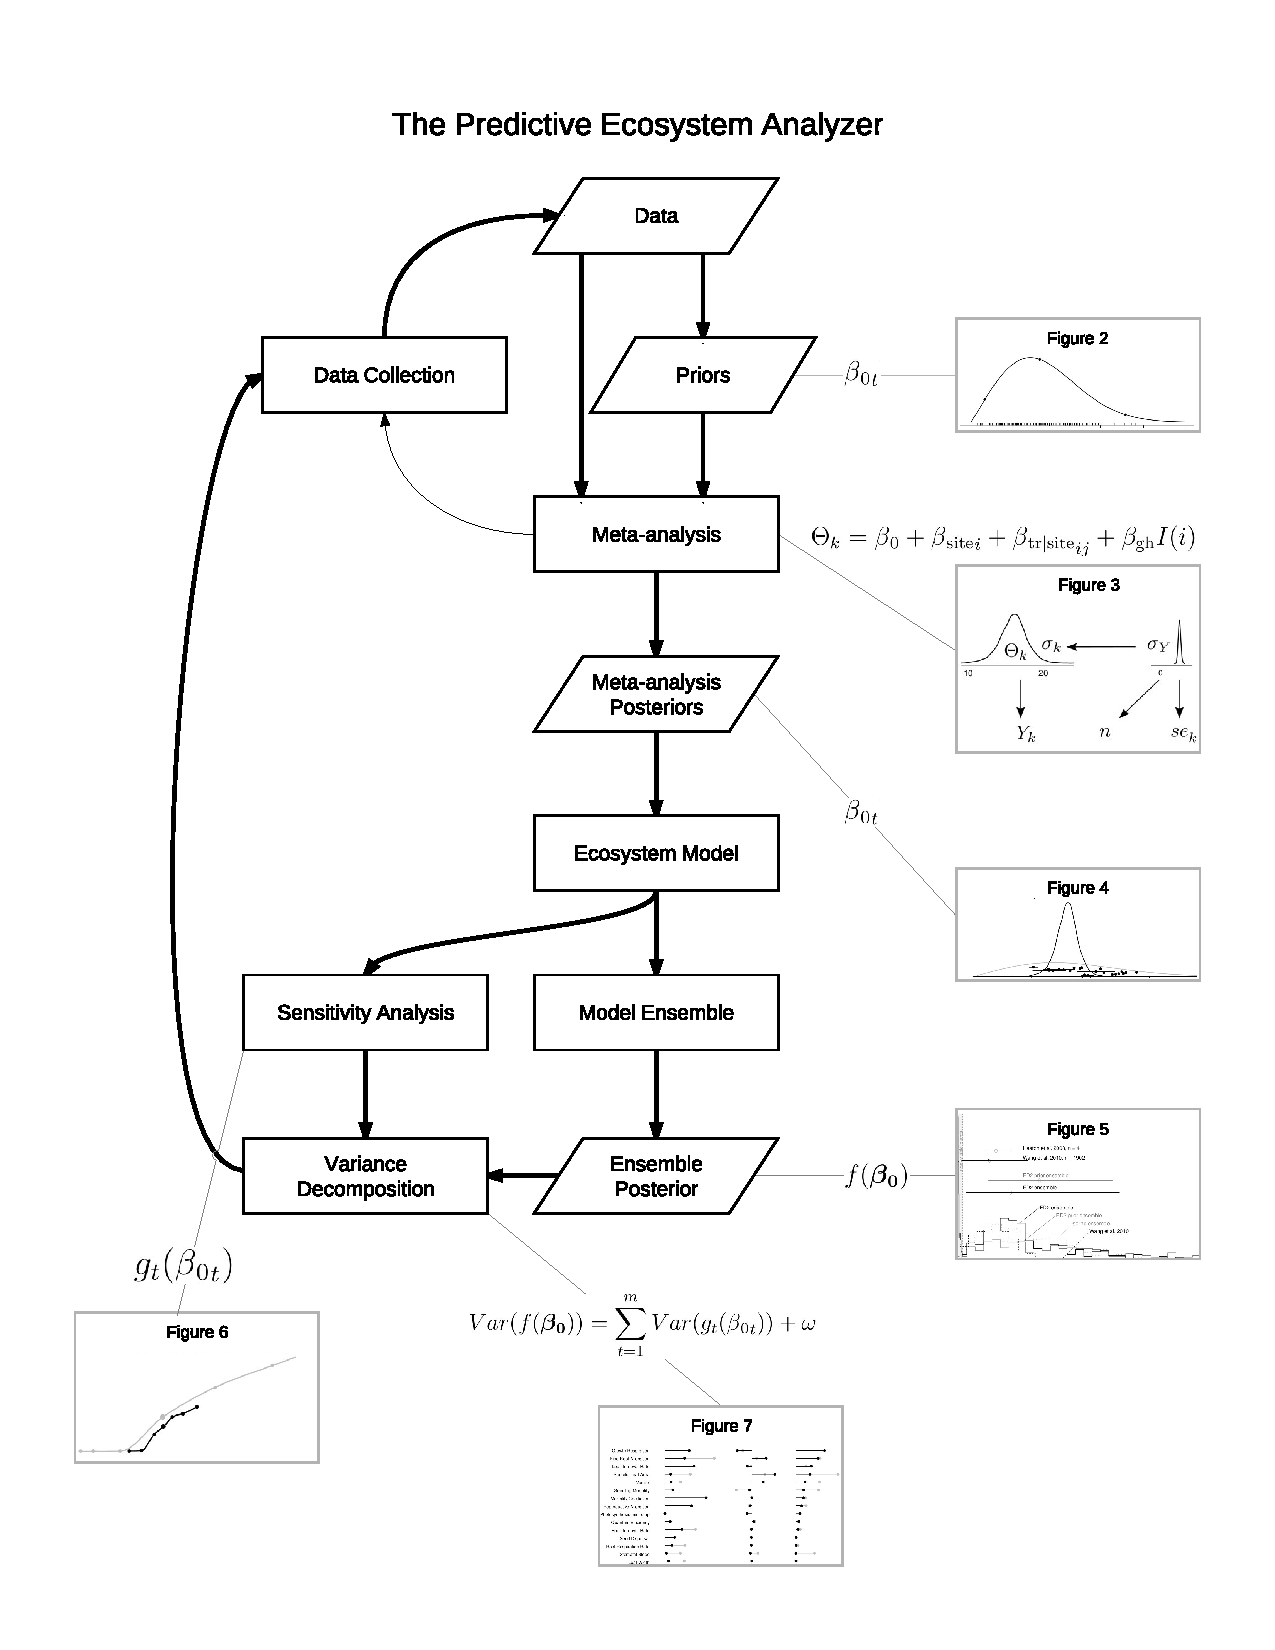
\includegraphics[width=0.8\textwidth]{workflow.pdf}
\end{center}
\label{fig:workflow}
\end{figure}



\begin{figure}
    \begin{centering}
    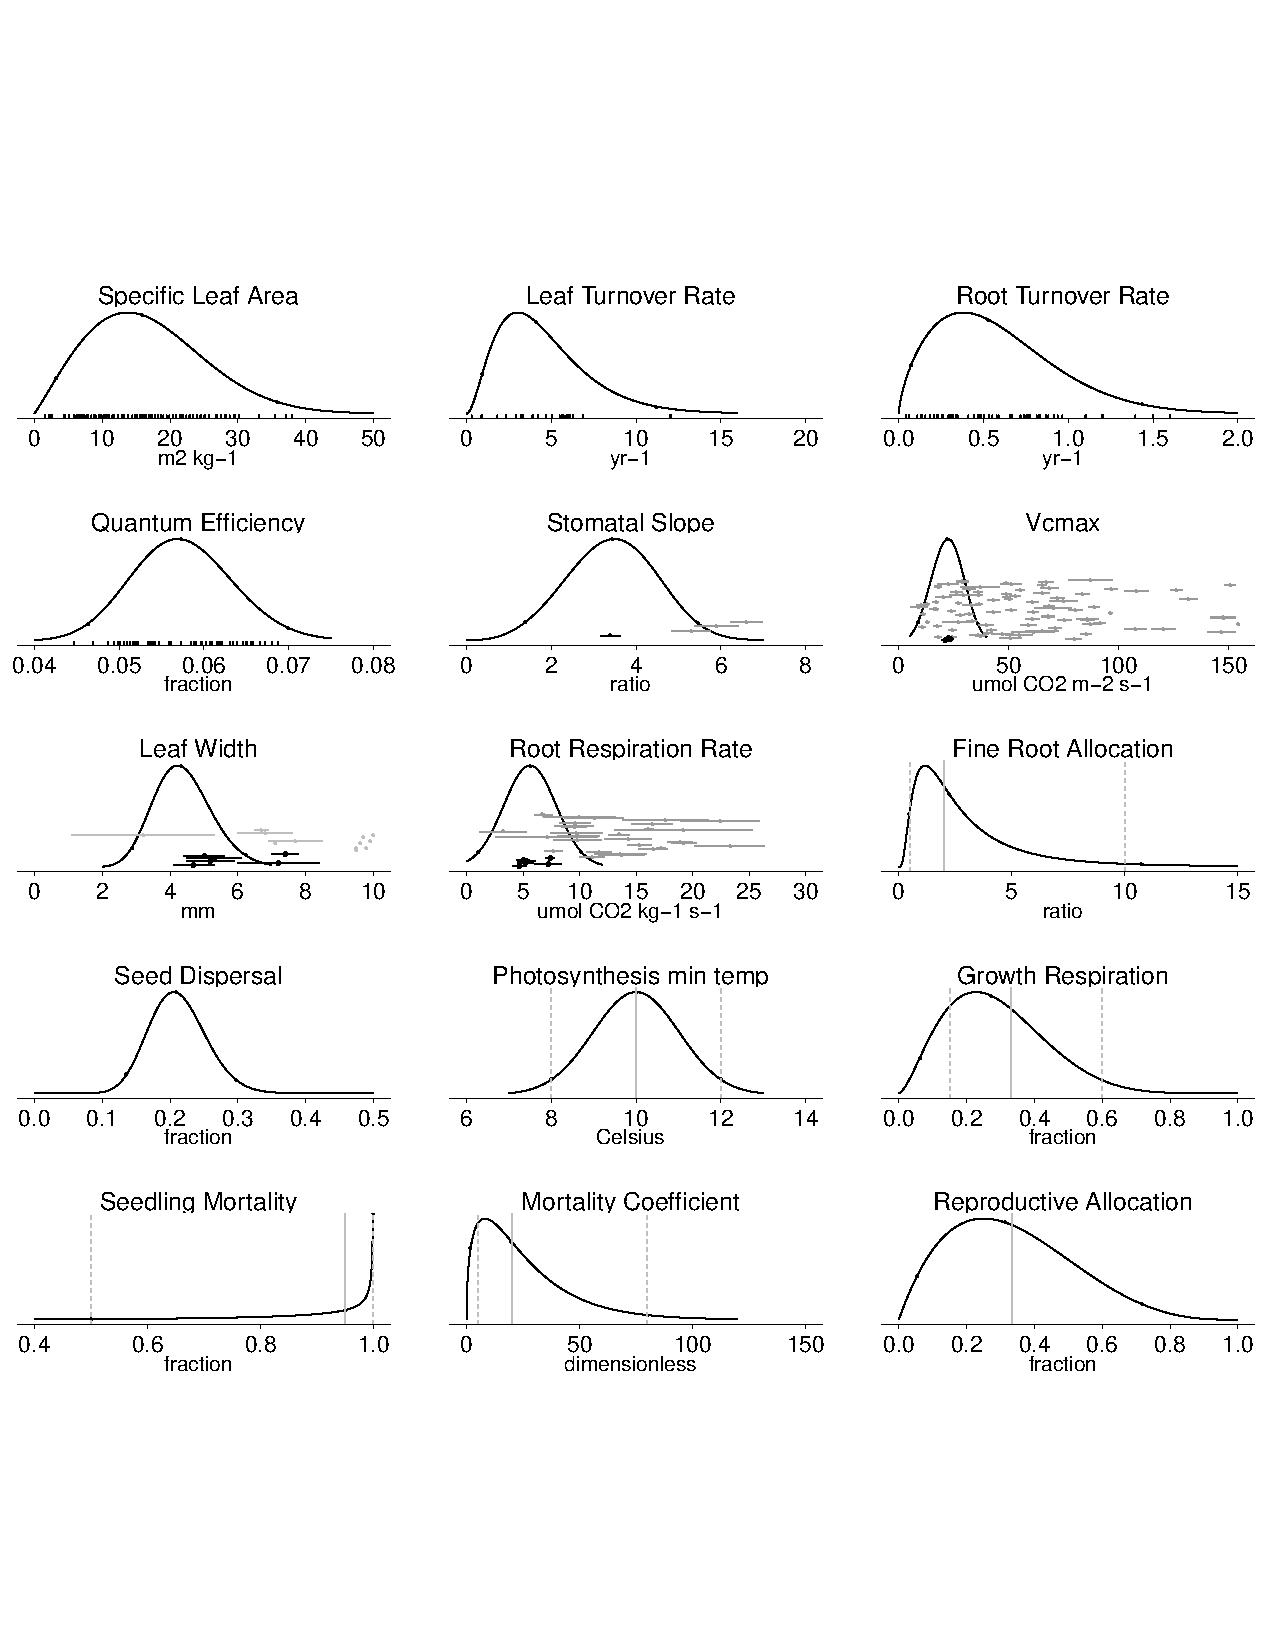
\includegraphics[width=6.5in]{priorfigures.pdf}
    \caption{{\bf Prior distributions} PDFs of priors with data constraints. 
      Parameter value is on the x-axis and probability density is on the y-axis, and the area under each curve equals one. 
      Three points on each line, from left to right, indicate the $2.5^{\text{th}}$, $50^{\text{th}}$, and $97.5^{\text{th}}$ quantiles. 
      (From top left) Four priors fit to data (data points shown as rug plot) using maximum likelihood: specific leaf area and leaf turnover rate \citep{wright2004wwl}, root turnover rate \citep{gill2000gpr}, and quantum yield \citep{skillman2008qyv}. 
      Four priors fit to the posterior predictive distribution of an unobserved C4 grass species using Bayesian meta-analysis of data from multiple plant functional types (C4 data shown in black, other functional types in grey): stomatal slope (present study data provided in Appendix A), V$_{\text{cmax}}$ of C3 plants \citep{wullschleger1993blc} and C4 grasses \citep{kubien2005ltp,massad2007etc,wang2011icp}, leaf width \citep{oyarzabal2008tdb}, and root respiration \citep{tjoelker2005llr}. 
      Priors fit to $95\%$ CI (dashed grey line) and median (solid grey line) based on ED2 defaults and expert opinion as described in the text: fine root to leaf ratio \citep{chapin2002pte}, seed dispersal (\citet{ernst1992pda} model parameterized with site level data), minimum temperature of photosynthesis (Don Ort, personal communication), growth respiration, seedling mortality factor, mortality factor, and reproductive allocation.}
    \label{fig:priors}
  \end{centering}
\end{figure}

\begin{figure}[p]
\caption%[Meta-analysis model]
{{\bf Overview of the Hierarchical Bayesian meta-analysis model.} 
  For each trait, the posterior estimate of the global trait mean ($\beta{_0}$) is used as an input parameter in the sensitivity analysis and model ensemble (Figures \ref{fig:agbsa} and \ref{fig:ensembledensity}). 
  Results from the meta-analysis of specific leaf area are as an illustrative example; x-axes have units of m$^2$kg$^{-1}$ and all plots are on the same scale.
 Each of the $k$ sample means ($Y_k$) are taken from published articles and unpublished field measurements, and may be associated with a sample standard error and sample size. 
 When sufficient data were available, site, treatment, and greenhouse effects were estimated.
 The within-unit standard deviation, $\sigma_Y$, is estimated from $se$ and $n$.
 Site and treatment random effects, represented by $\beta_{\text{site}}$ and $\beta_{\text{tr|site}}$, are estimated for each site and treatment within site with from normal distributions with mean zero and standard deviations $\sigma_{\text{site}}$ and $\sigma_{\text{tr|site}}$, respectively. 
 Greenhouse is a fixed effect.
 Table \ref{tab:maresults} summarizes the global mean, variance terms, and greenhouse effect for the seven model parameters informed by species-level data.
  }
\begin{center}
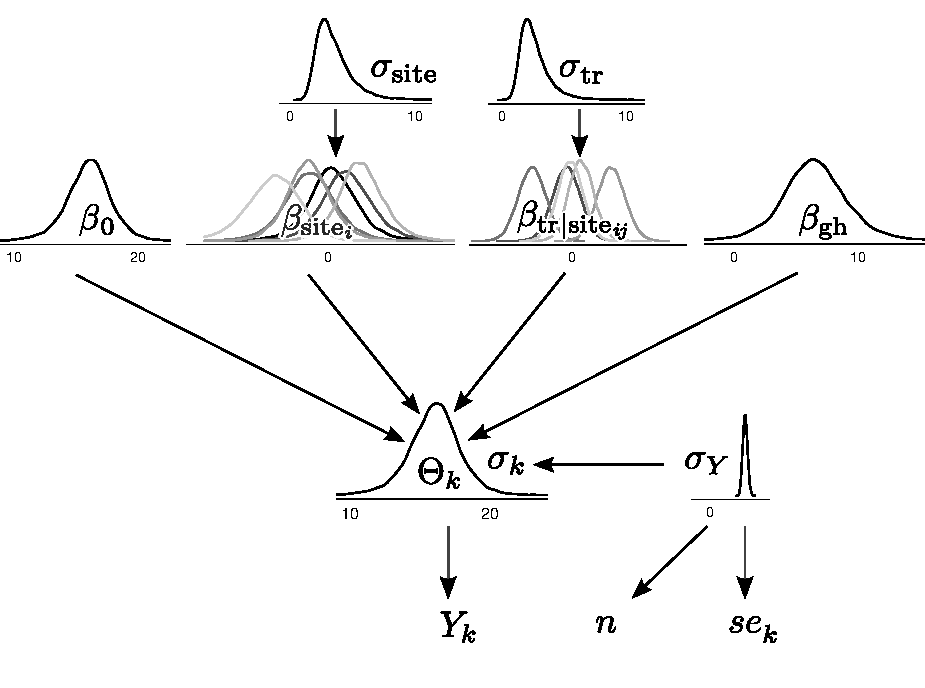
\includegraphics{mamodel.pdf}
\end{center}
\label{fig:ma}
\end{figure}


\begin{figure}[p]
  \caption%[Trait priors and posteriors]
{{\bf Prior (gray) and posterior (black) densities of trait parameters used in the analysis.} 
    Priors distributions are based on the traits of plants within broad taxonomic or functional type groupings (e.g. all grasses). 
    When species-level data were available, they are used in a hierarchical Bayesian meta-analysis, and the posterior estimate of the mean parameter value is shown. 
    Data used in the meta-analysis come from both published and direct measurements of the trait on the perennial C4 grass Switchgrass (\emph{Panicum virgatum}).
    These data are represented as mean $\pm$SE.
    Mismatch between data and the posterior estimate of the global trait mean results from site, treatment, and greenhouse effects. 
    Data from plants grown under an experimental treatment or in a controlled environment (e.g. in a pot or greenhouse) are presented in grey; data from field-grown plants under control treatments are in black. 
Site-level effects account for disparity between raw data and parameter distribution in the SLA and leaf width plots.
}
\begin{center}
  \includegraphics[width=0.9\textwidth]{traitpdfs.pdf}
\end{center}
  \label{fig:traitpdfs}
\end{figure}


\begin{figure}[p]
\caption%[Ensemble Yields]
{{\bf Ensemble average 2004-2006  post-senescence yield.} 
  Histogram of results from prior ensemble runs (dashed), posterior ensemble runs (solid line), and the spline ensemble (gray line).  
  The gray box on the left represents non-viable ensemble members ($\leq 2\text{Mg/ha}$, see text).
  Horizontal bars provide a summary of yields, from top: a three year trial at the modeled site \citep{heaton2008mub},  all $1902$ observations included in a recent meta-analysis \citep{wang2010qrc}, viable runs from the ED2 ensemble based on prior and posterior parameterizations.
  Diamonds indicate the median; thick and thin lines indicating the $68\%$ and the $95\%$ CI, respectively.
  Histogram-style plots provide comparison of the distributions of observations and model runs.
  For clarity, non-viable and viable runs are plotted with different width bins.
} 
\begin{center}
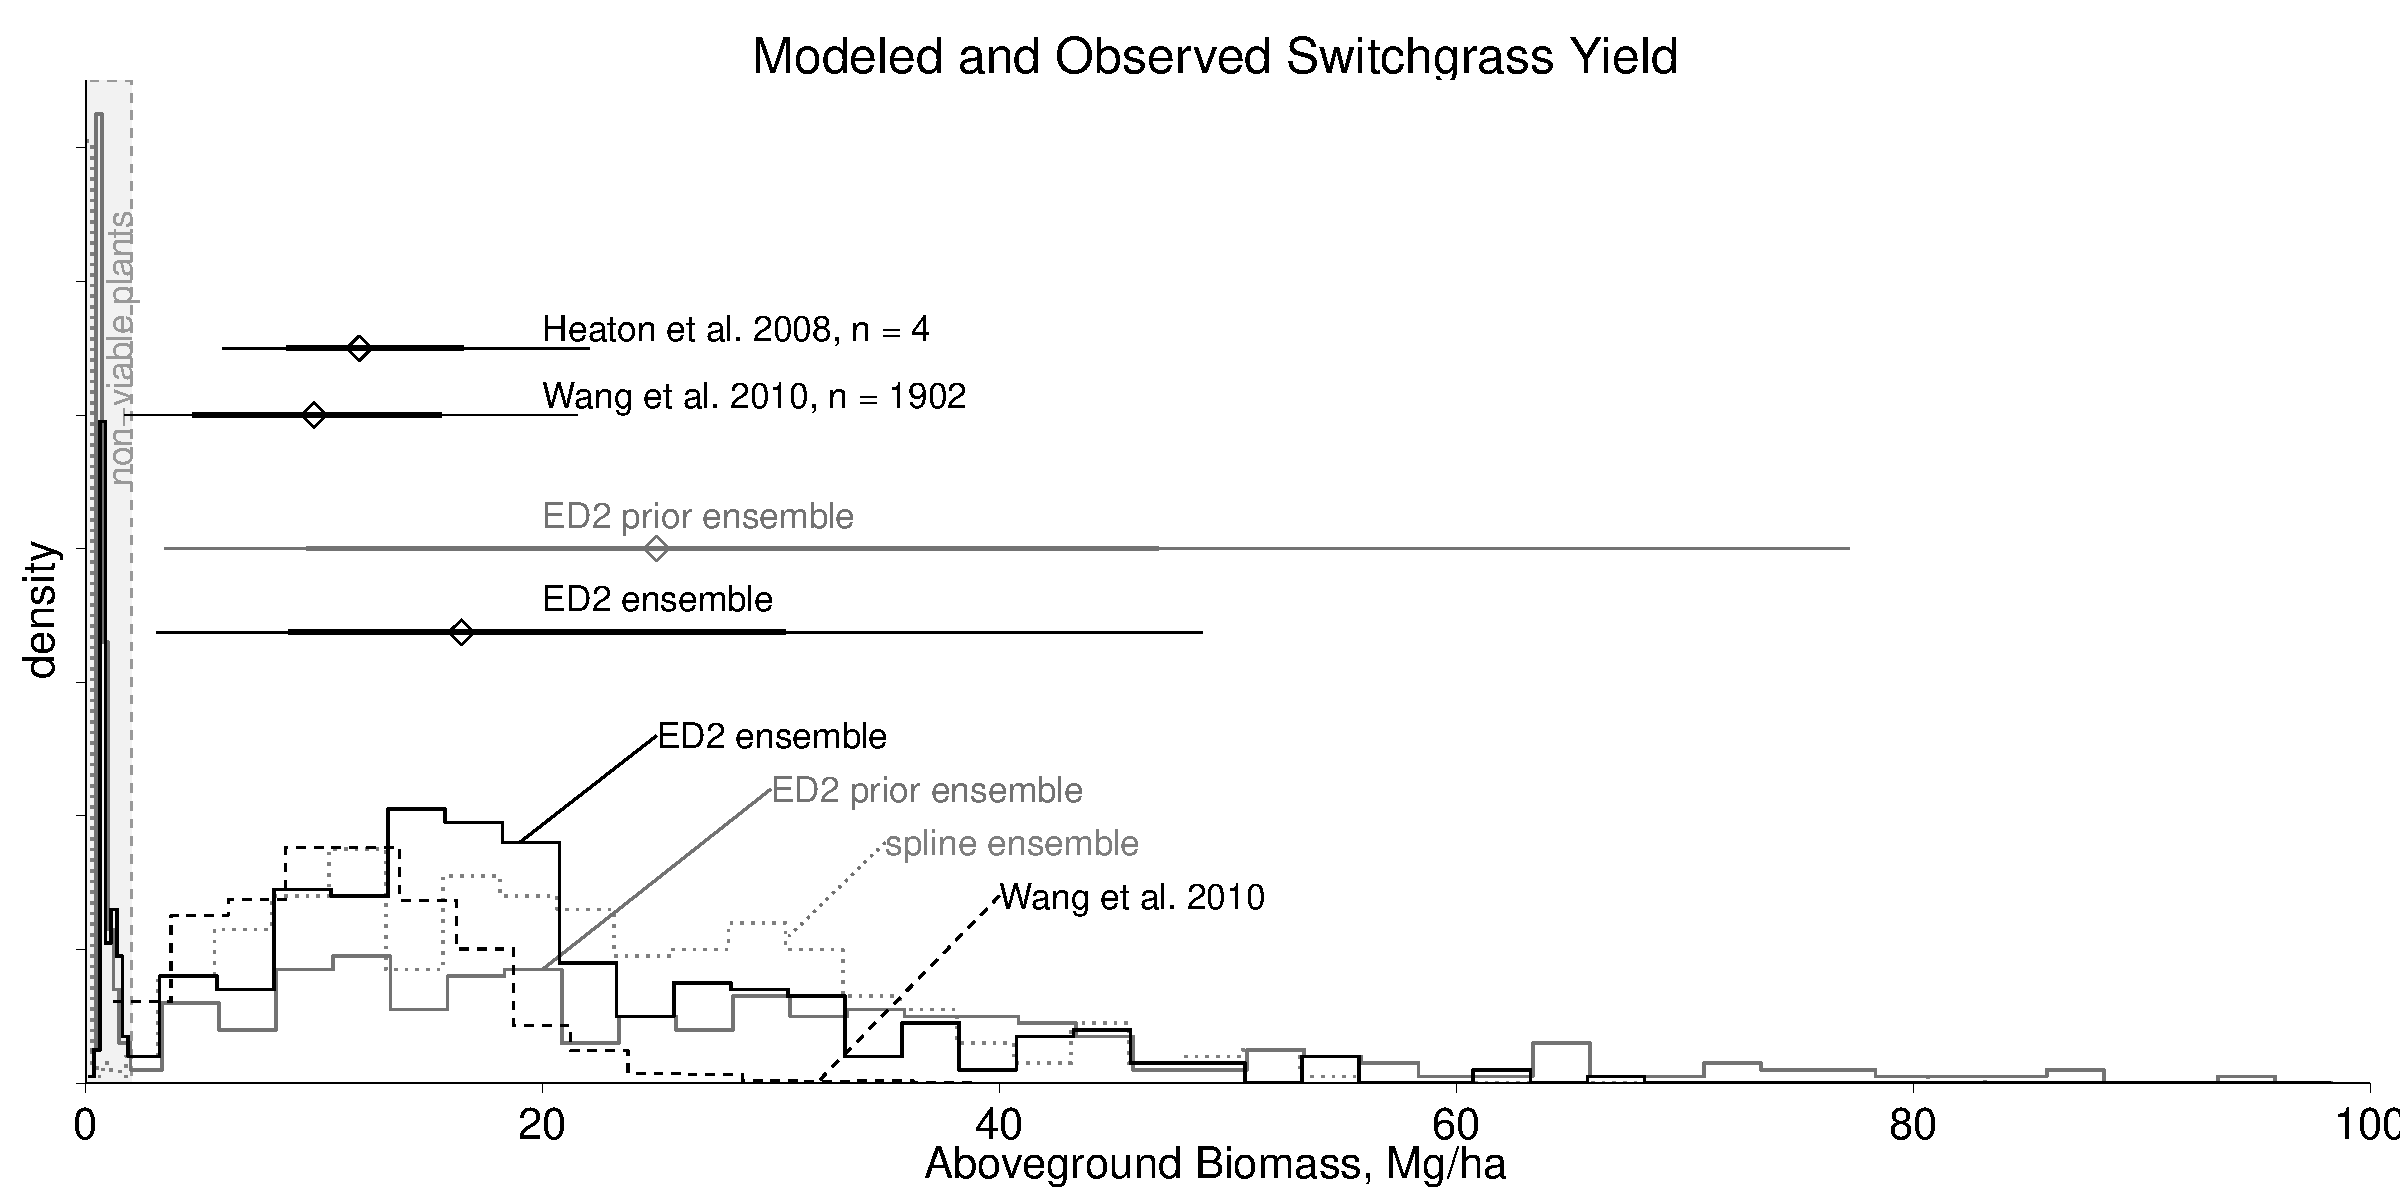
\includegraphics[width=\textwidth]{ensembledensity.pdf}
\end{center}
\label{fig:ensembledensity}
\end{figure}

\begin{figure}[p]
  \caption%[Sensitivity Analysis Plots]
  {{\bf Univariate relationships between parameters and 2004-2006 average modeled yield.} Parameter values are on the x-axis and biomass is on the y-axis while runs centered around the prior median are in gray and those centered around the posterior median are in black. The univariate responses were estimated using a cubic spline to fit model output at the median and $\pm[1,2,3]\sigma$ quantiles of each parameter while holding other parameters to the median value.}
  \begin{center}
    \includegraphics[width=0.9\textwidth]{sensitivityanalysisplotslabel.pdf}
  \end{center}
  \label{fig:agbsa}
\end{figure}



\begin{figure}[p]
\caption%[Variance Decomposition]
{{\bf Partitioning of variance by parameter} results from variance decomposition conducted before (grey) and after (black) updating parameter estimates with species-level data in the meta-analysis.
 From left to right, panels present: a) the uncertainty associated with each parameter (coefficient of variation, $\text{CV}=\sigma/\mu$).
 The degree to which some parameters have been constrained by data is indicated by the reduction in CV in the black compared to the grey bars; sample sizes are indicated in Table~\ref{tab:maresults}.
  b) the sensitivity of modeled aboveground biomass to each parameter presented as elasticity (elasticity is normalized sensitivity, and an elasticity of one indicates that model output will double when the parameter value doubles).
  Sensitivity is the slope of the line at the median in Figure~\ref{fig:agbsa}). 
  Parameters with larger bars have greater influence on model output.
  c) Partial variance is the contribution of each parameter to explained variance. 
  This is a function of both the parameter variance and sensitivity. 
  Parameters with both large CV and elasticity contribute the most to uncertainty in model output.}
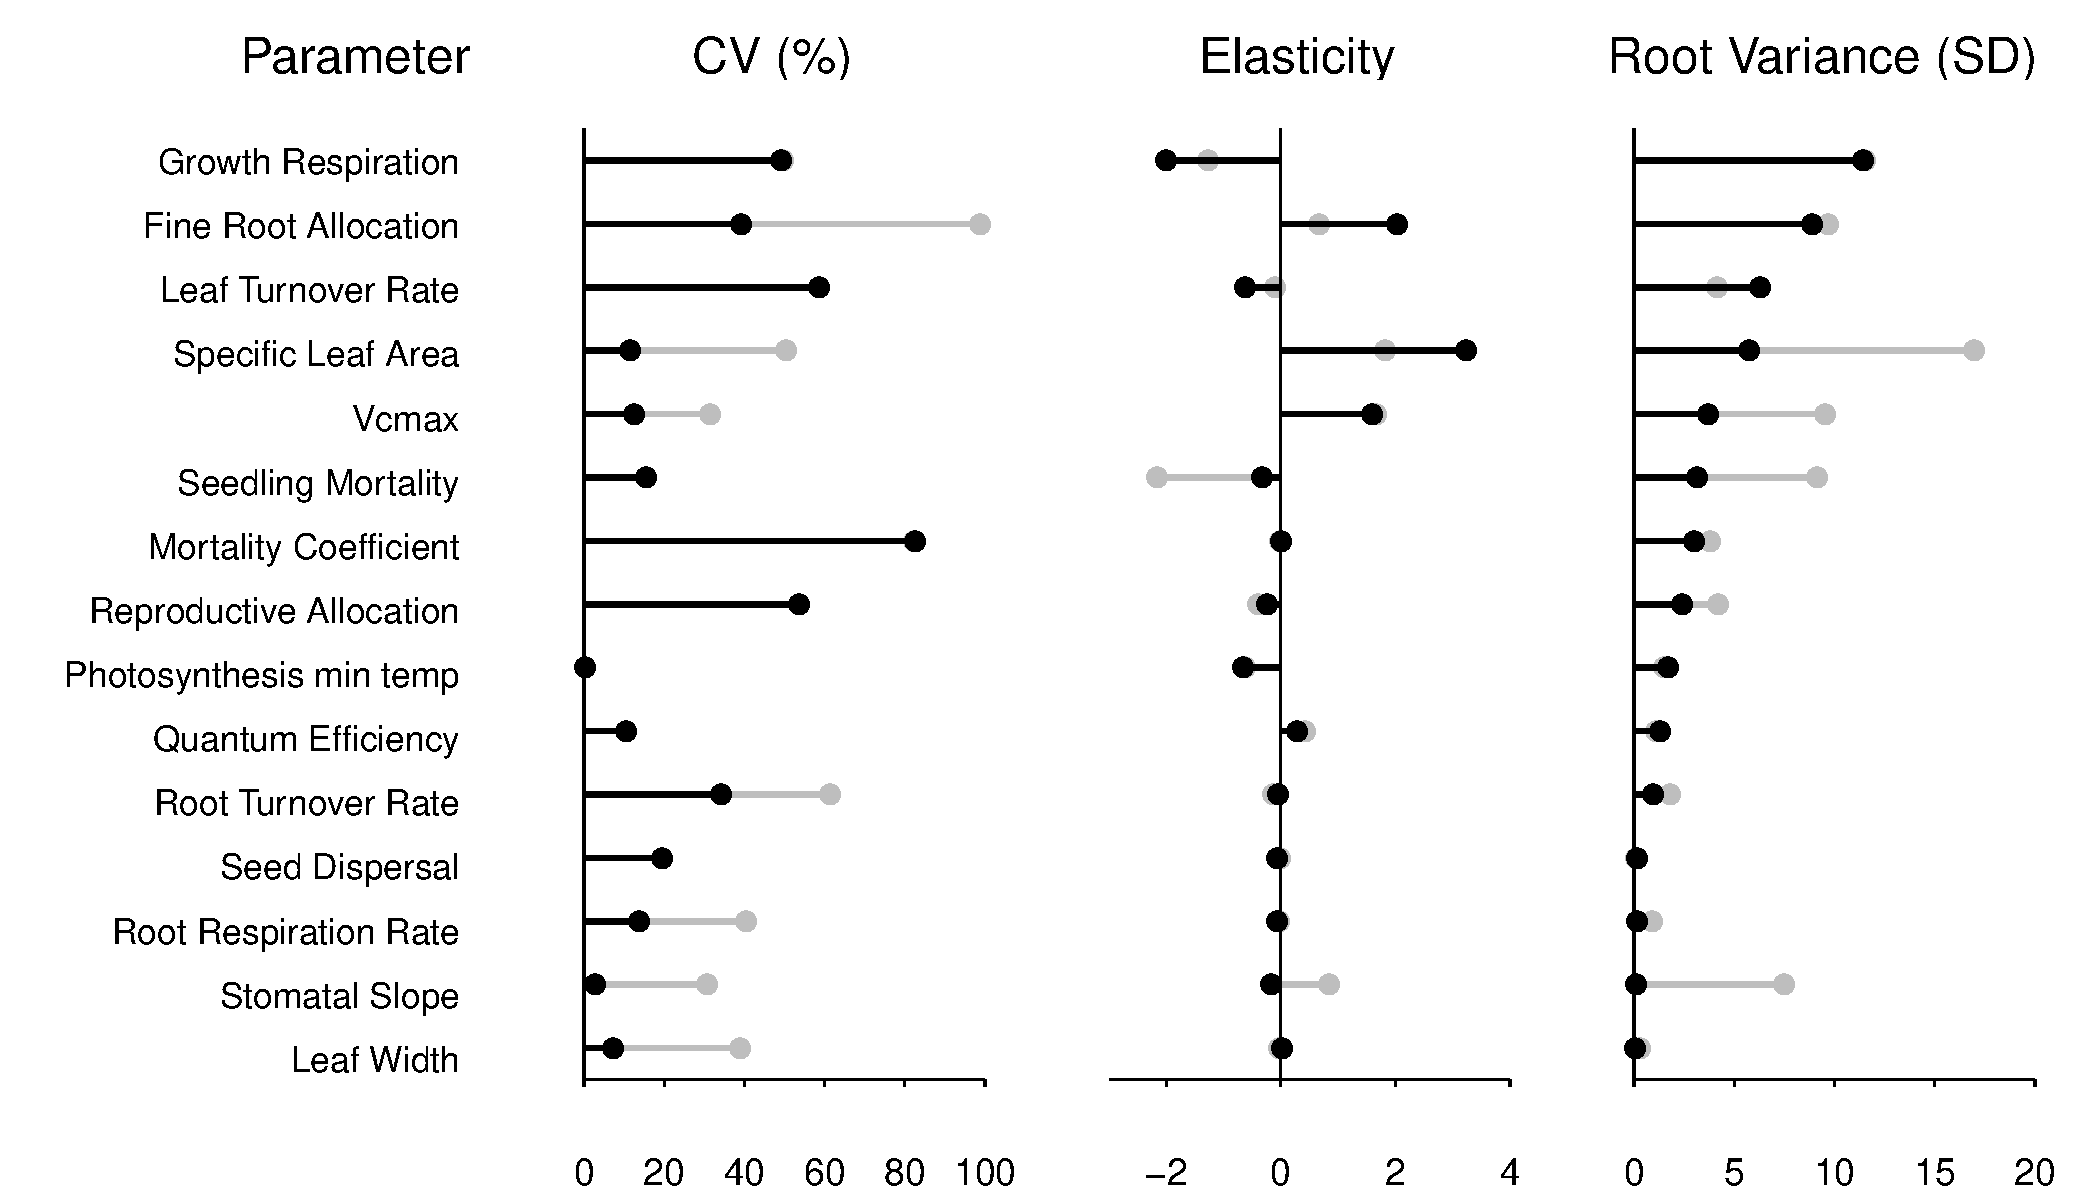
\includegraphics[width=\textwidth]{variancedecomposition.pdf}
\label{fig:vd}
\end{figure}

\clearpage
%\processdelayedfloats

%\appendix
%\documentclass[12pt]{article}

%% Math
\usepackage{amsmath}  % for math formulas
\usepackage{amssymb}  % for math symbols
\usepackage{bm}
\renewcommand{\vec}[1]{\bm{#1}} %% define vector notation

%% Tables
\usepackage{rotating} % enable sidewaystable
\usepackage{longtable} % used for long tables of data in appendix
\usepackage{booktabs}  % also for long tables of data in appendix
\usepackage{subfig}
%% Figures
\usepackage{graphicx}
%% all fig. legends on a separate page
%% http://tex.stackexchange.com/q/30477/1783
\usepackage{caption}
\usepackage{letltxmacro}% http://ctan.org/pkg/letltxmacro
\captionsetup{labelsep=none}
\DeclareCaptionTextFormat{none}{} \captionsetup{labelsep=none,textformat=none}

%% Text layout
\usepackage{setspace} 
\usepackage{geometry}
\geometry{verbose,a4paper,tmargin=2.4cm,bmargin=2.4cm,lmargin=2.4cm,rmargin=2.4cm}
\usepackage{lineno}
\linenumbers
\usepackage{Sweave}% use of Sweave with R code
\usepackage{natbib}
\bibliographystyle{ecology}

\title{Appendix}
\date{} % Leave date blank
\begin{document}

\begin{flushleft}
\begin{spacing}{1.9}


\section{Switchgrass Data}
\end{spacing}
\begin{spacing}{1}
\label{app:data}
All data used in the present analysis, along with site, citation, and treatment information, are available in the BETY database. Each data point is identified by a unique trait\_id: id is the primary key in the traits table, and trait\_id is the foregin key in auxillary tables (Appendix B).

\subsection*{Present study data}
 
\subsubsection*{Vcmax and SLA}
V$_{\text{cmax}}$ and SLA measurements were made on four year old switchgrass (\emph{P.~virgatum}) stands were grown in an agricultural study site in Savoy, IL (40$^o$10'20"N, 88$^o$11'40"W, 228 m above sea level).
Gas exchanges were measured on leaves with a portable infrared gas analyzer (LI-COR 6400LCF; Li-COR, Lincoln, NE). 
During measurements, leaves were exposed to a CO$_2$ concentration of 370 $\mu$mol mol$^{-1}$, temperature at $25^o$C, vapor pressure deficit (VPD) at the leaf surface 1.5 kPa and airflow through the chamber 250 $\mu$mol s$^{-1}$. For the CO$_2$ response (A-Ci) curves, leaves were acclimated for 30-60 minutes before adjusting the CO$_2$ concentrations. 
Thereafter, CO$_2$ concentration was decreased in 5 steps (400, 300, 200, 100 and 50 ppm CO$_2$) and then increased in 3 steps (400, 600 and 800 μmol mol-1 CO$_2$). A-Ci curves were fitted to a coupled photosynthesis-stomatal conductance model \citep{collatz1992cps}. 
The rate saturated region of the A-Ci curves were used to estimate maximum Rubisco activity (Vcmax) \citep{miguez2009smp}. 

SLA was computed as the ratio of leaf area to mass. Ten 0.5 cm$^2$ leaf punches from 4 different plants were taken and oven-dried at 65 $^o$C for two weeks and then weighed.

\subsubsection*{Stomatal Slope data}

Stomatal slope was estimated using measurements of four leaves from each of five field-grown energy crop species during the 2010 growing season. 
The five species included two C4 grasses: Miscanthus (\textit{Miscanthus~x~giganteus}) and Switchgrass (\textit{P~virgatum}) planted in 2008 and three deciduous tree species: Red Maple (\textit{Acer~rubrum}), Eastern Cottonwood (\textit{Populus~deltoides}, and Sherburne Willow \textit{Salix~x~Sherburne}) planted in 2010 as 2 year old saplings. 
 All plants were grown at the Energy Biosciences Institute Energy Farm (40$^o$10'N, 88$^o$03"W).

Photosynthesis (A), stomatal conductance (gs), intercellular [CO$_2$] (ci), and humidity deficit at the leaf surface (Ds) were obtained via open gas exchange systems with 2 cm$^2$ leaf chambers housing infrared gas analyzers to measure fluxes of both CO$_2$ and water (LI-6400; LI-COR Inc., Lincoln, NE, USA). 
Data were collected following a simplified version of the protocol described by \citet{leakey2006ltg} in which photosynthetic photon flux density was maintained at 1500 $\mu$mol m$^{-2}$ s$^{-1}$, leaf temperature was $25 \pm 3^o$C and the vapor pressure deficit from leaf to air was < 2 kPa while [CO$_2$] entering the chamber was varied stepwise (400, 250, 350, 450, 650, 850, 1200, 1500 ppm). A minimum of 20 minutes was allowed for A and gs to completely stabilize before data were collected at each [CO$_2$]. 
 For each individual leaf, linear least squares regression was used to estimate the stomatal slope based on the \citet{ball1987mps} model of stomatal conductance (not used in present study but provided as data in appendix), and then separately for the \citet{leuning1995cac} model of stomatal conductance. A common value of $\Gamma=40 \mu$P Pa$^{-1}$, and D$_0=1500$ Pa was used in accordance with \citet{leuning1995cac}.

{\small
\begin{longtable}{rrrlr}
  \toprule
  Mean & n & SE & BETY trait\_id \\
  \midrule \endhead
  Leuning slope parameter & & & & \\*
  \hline
  4.35& 1& 	0.51 & 40909\\
  3.93& 1& 	0.13 & 40910\\
  3.74& 1& 	0.21 & 40911\\
  4.37& 1& 	0.33 & 40912\\
  \hline
  SLA ($g C/ m^2$) & & & & \\*
  \hline
  34.5 &  2 & 12.2  & 2592 \\* 
  28.4 &  2 & 4.7  & 2593 \\* 
  32.1 &  2 & 3.6  & 2597 \\* 
  30.5 &  2 & 5.7  & 2598 \\* 
  \hline
  Vcmax & & &  \\*
  \hline
  18.1 &  2 & 6.2 & 2638 \\* 
  16.3 &  2 & 2.9 & 2639 \\* 
  8.9 &  2 & 4.8  & 2640 \\* 
  8.8 &  2 & 6.97 & 2641 \\* 
  20.8 &  2 & 7.5 & 2642 \\* 
  14.4 &  2 & 5.8 & 2643 \\* 
  16.9 &  2 & 8.4 & 2644 \\* 
  6.2 &  2 & 2.1  & 2645 \\
  \hline
  \bottomrule
  \caption{ Unpublished switchgrass trait data collected for the present analysis.}
\end{longtable}
}
\newpage
\subsection*{Previously published data}
\begin{longtable}{rrrlr}
  \toprule
  Mean & n & SE & citation & BETY trait\_id \\
  \midrule \endhead
  SLA ($g C/ m^2$) & & & & \\*
  \hline
  38.8 &  2 & 1.0 & \citet{knapp1995efd} & 132 \\* 
  40.6 &  2 & 2.2 & \citet{knapp1995efd} & 133 \\* 
  40.8 &  8 &  & \citet{byrd2000pcs} & 281 \\* 
  39.6 &  8 &  & \citet{byrd2000pcs} & 282 \\* 
  49.5 &  8 &  & \citet{byrd2000pcs} & 283 \\* 
  51.7 &  4 &  & \citet{byrd2000pcs} & 285 \\* 
  53.3 &  4 &  & \citet{byrd2000pcs} & 286 \\* 
  46.4 &  4 &  & \citet{byrd2000pcs} & 287 \\* 
  54.2 &  4 &  & \citet{byrd2000pcs} & 288 \\* 
  58.0 &  4 &  & \citet{byrd2000pcs} & 289 \\* 
  52.8 &  4 &  & \citet{byrd2000pcs} & 290 \\* 
  45.2 &  4 &  & \citet{trocsanyi2009ycc} & 8478 \\* 
  37.9 &  4 &  & \citet{trocsanyi2009ycc} & 8482 \\* 
  38.5 &  4 &  & \citet{trocsanyi2009ycc}  & 8487 \\
  \hline
  \hline
  fine root:leaf & & & &  \\*
  \hline
  0.59 &  4 &  & \citet{kiniry1999rue} & 22092 \\* 
  2.73 &  4 &  & \citet{kiniry1999rue} & 22093 \\* 
  0.43 &  4 &  & \citet{kiniry1999rue} & 22094 \\* 
  1.5 &  4 &  & \citet{kiniry1999rue}  & 22095 \\* 
  1.81 &  2 & 0.27 & \citet{tjoelker2005llr} & 25670 \\* 
  0.74 &  2 & 0.30 & \citet{tjoelker2005llr} & 25675 \\
  \hline

  \newpage
  \hline
  leaf width (mm) & & & & \\*
  \hline
  10.2 & 2 & 0.27 & \citet{knapp1995efd} & 136 \\* 
  5.9 &  2 & 0.23 & \citet{knapp1995efd} & 137 \\* 
  5.0 &  2 & 0.18 & \citet{redfearn1997cam} & 332 \\* 
  4.9 &  2 & 0.18 & \citet{redfearn1997cam} & 333 \\* 
  6.4 &  2 & 0.18 & \citet{redfearn1997cam} & 334 \\* 
  6.3 &  2 & 0.18 & \citet{redfearn1997cam} & 335 \\* 
  6.2 &  2 & 0.18 & \citet{redfearn1997cam} & 336 \\* 
  7.2 &  2 & 0.18 & \citet{redfearn1997cam} & 337 \\* 
  5.2 &  2 & 0.18 & \citet{redfearn1997cam} & 338 \\* 
  4.6 &  2 & 0.18 & \citet{redfearn1997cam} & 339 \\* 
  6.2 &  2 & 0.18 & \citet{redfearn1997cam} & 340 \\* 
  5.8 &  2 & 0.18 & \citet{redfearn1997cam} & 341 \\* 
  4.6 &  2 & 0.18 & \citet{redfearn1997cam} & 342 \\* 
  6.8 &  2 & 0.18 & \citet{redfearn1997cam} & 343 \\* 
  6.8 &  2 & 0.18 & \citet{redfearn1997cam} & 344 \\* 
  6.6 &  2 & 0.18 & \citet{redfearn1997cam} & 345 \\* 
  7.9 &  2 & 0.18 & \citet{redfearn1997cam} & 346 \\* 
  7.4 &  2 & 0.18 & \citet{redfearn1997cam} & 347 \\* 
  6.7 &  2 & 0.18 & \citet{redfearn1997cam} & 348 \\* 
  7.0 &  2 & 0.18 & \citet{redfearn1997cam} & 349 \\* 
  4.8 &  2 & 0.18 & \citet{redfearn1997cam} & 386 \\* 
  4.8 &  2 & 0.18 & \citet{redfearn1997cam} & 387 \\* 
  6.2 &  2 & 0.18 & \citet{redfearn1997cam} & 388 \\* 
  5.8 &  2 & 0.18 & \citet{redfearn1997cam} & 389 \\* 
  4.7 &  2 & 0.18 & \citet{redfearn1997cam} & 390 \\* 
  7.7 &  2 & 0.18 & \citet{redfearn1997cam} & 391 \\* 
  4.6 &  2 & 0.18 & \citet{redfearn1997cam} & 392 \\* 
  5.6 &  2 & 0.18 & \citet{redfearn1997cam} & 393 \\* 
  7.3 &  2 & 0.18 & \citet{redfearn1997cam} & 394 \\* 
  6.6 &  2 & 0.18 & \citet{redfearn1997cam} & 395 \\* 
  7.3 &  2 & 0.18 & \citet{redfearn1997cam} & 396 \\* 
  7.0 &  2 & 0.18 & \citet{redfearn1997cam} & 397 \\* 
  5.1 &  2 & 0.18 & \citet{redfearn1997cam} & 398 \\* 
  4.7 &  2 & 0.18 & \citet{redfearn1997cam} & 399 \\* 
  5.8 &  2 & 0.18 & \citet{redfearn1997cam} & 400 \\* 
  6.4 &  2 & 0.18 & \citet{redfearn1997cam} & 401 \\* 
  5.0 &  2 & 0.18 & \citet{redfearn1997cam} & 402 \\* 
  7.0 &  2 & 0.18 & \citet{redfearn1997cam} & 403 \\* 
  7.6 &  2 & 1.70 & \citet{oyarzabal2008tdb} & 453 \\ 
  \hline
  \caption{ Previously published switchgrass trait data used in meta-analysis}
\end{longtable}
\newpage

\section{BETYdb}
\label{app:betydb}

 The Biofuel Ecophysiological Traits and Yields database (BETYdb, http://ebi-forecast.igb.uiuc.edu) structure (Figure \ref{fig:betydbschema}). Comprehensive documentation of database structure and web-based data entry is available at the website.

\begin{figure}[ht!]    
 \includegraphics[width=3in]{betydbschema}
 \caption{ Database schema for the traits database.}
 \label{fig:betydbschema}
\end{figure}

\clearpage
\section{Transformations}

% \subsection{Unit conversions}

% The following non-standard conversions were used to convert data from reported units to the standardized units used in BETYdb. 
% \begin{table}[ht]
%   \caption{Unit conversions}
%   \label{tab:traitconversion}
%   \begin{tabular}{lllp{2in}}
%     \hline
%     from ($X$) & to ($Y$) & conversion                      & notes\\ \hline
%      $X_1=$biomass, $X_2=$production & root turnover rate & $Y = X_2/X_1$&  \citet{gill2000gpr}\\
%     US ton/acre &Mg/ha &$Y = X * 2.24$ & \\
%     \% roots &root:shoot (q)& $Y=\frac{X}{1-X}$& $\% \text{roots} = \frac{\text{root biomass}}{\text{total biomass}}$ \\
%     mm s$^{-2}$&mmol m$^{-3}$ s$^{-1}$ &$Y=X/41$ &\citet{korner1988gsc} \\
%     mg CO$_2$ g$^{-1}$ h$^{-1}$ & $\mu$mol kg$^{-1}$ s$^{-1}$& $Y = X\times 6.31$& root respiration rate\\
%     \hline
%   \end{tabular}
% \end{table}


\subsection*{Arrhenius correction}\label{app:arrhenius}
 Parameters for enzyme kinetics ($V_{c_{max,T_m}}$ and root respiration rate) were scaled from the measurement temperature ($T_o$) to a standard temperature ($T_m=298 K (= 25^oC)$) using an Arrhenius correction:
$$V_{c_{max,T_m}}=\frac{V_{c_{max,T_0}}}{e^{3000*(1/(T_o)-1/(T_m))}}$$  

\subsection*{Estimating SE from reported statistics}\label{app:seest}

Often, differences between treatments are reported with P-values, least significant differences (LSD), and other statistics but provide no direct estimate of the variance.
It is reasonable to always assume that the statistics were calculated using the assumption that the data are normally distributed.

\begin{enumerate}
\item given MSE and $n$
 $$SE=\sqrt{MSE/n}$$
\item given $P$, $n$, and treatment means $\bar X_1$ and $\bar X_2$

$$SE=\frac{\bar X_1-\bar X_2}{t_{(1-\frac{P}{2},2n-2)}\sqrt{2/n}}$$

\item given LSD, $\alpha$, $n$, $b$ where $b$ is number of blocks $^{1}$, and $n=b$unless otherwise specified for a randomized complete block design \citep{rosenberg2004map}:

$$SE = \frac{LSD}{t_{(0.975,n)}\sqrt{2bn}}$$

\item given MSD (minimum significant difference) given $n$, $\alpha$, df = $2n-2$  \citep{wang2000asp}

$$SE = \frac{MSD}{t_{(0.975, 2n-2)}\sqrt{2}}$$

\item given a 95\% Confidence Interval (measured from mean to upper or lower confidence limit), $\alpha$, and $n$  \citep{saville2003bsi}
$$SE = \frac{CI}{t_{(\alpha/2,n)}}$$
\item given Tukey's HSD, $n$, where $q$ is the `studentized range statistic', $$SE = \frac{HSD}{q_{(0.975,n)}}$$
\item To solve for $MSE$ given $F$, $df_{\textrm{group}}$, and $SS$ (required when a partial anova table is provided)
The definition $F = MS_g/MS_e$, where $g$ indicates the group, or treatment can be rearranged to solve for the MSE: $MS_e=MS_g/F$
 Then if $MS_x = SS_x/df_x$, we can substitute $SS_g/df_g$ for $MS_g$ in the definition of $F$: $F=\frac{SS_g/df_g}{MS_e}$ and then solve for $MS_e$: $MS_e = \frac{SS_g}{df_g\times F}$.

\end{enumerate}
 In the present study, all required transformations were done prior to entry in the database using these formulas. 
 Subsequently, the PEcAn function \texttt{transformstats} has been developed to automate transformations of SD, MSE, LSD, 95\%CI, HSD, and MSD to conservative estimates of SE.

\subsection*{Calculating precision from SE}

Given variance ($\sigma^2=\frac{1}{N}\sum(i_i-\mu)^2$), sd $\left(\sigma=\sqrt{\sigma^2}=\sqrt{\frac{1}{N}\sum(i_i-\mu)^2}\right)$, and se ($se=\frac{\sigma}{\sqrt{n}}$), calculate precision $\tau$:

$$\sigma=se*\sqrt{n}$$
$$\sigma^2=se^2*n$$
$$\tau=\frac{1}{\sigma^2}=\frac{1}{se^2*n}$$

\section{Derivation of a Gamma prior on $\tau$}

$$\tau \sim G(\frac{n}{2}, \frac{\sum_{i=1}^{n}(\mu-x_i)^2}{2})$$

$$1/\tau_0=\sigma^2=\frac{\sum_{i=1}^{n}(\mu-x_i)^2}{n}$$

$$n/\tau_0=n\sigma^2=\sum_{i=1}^{n}(\mu-x_i)^2$$
  
$$\tau \sim IG(\frac{n}{2}, \frac{n}{2\tau})$$

\newpage
\bibliography{pecan_manuscript}
\end{spacing}
\end{flushleft}
\end{document}

\end{spacing}
\end{flushleft}
\end{document}

 
